\chapter{The Standard Model and Beyond}\label{ch:theory}
In this chapter we provide the theoretical basis for our analysis. The first section discusses the standard model (SM), which provides the best description of particle phenomena up to today. Despite its known success, there are energy domains in which the SM shows its limitations. In this light, extensions to the theory collectively known as Beyond Standard Model Physics, are proposed. We talk more about these limitations in Section~\ref{sec:SMLimitations}. In Section~\ref{sec:BSMNonReso}, we discuss three BSM extensions to the Standard Model, the ADD Large Extra Dimensions~\ref{sec:ADDmodel}, the Clockwork Model~\ref{sec:CWmodel} and the Unparticles~\ref{sec:UnparticlesModel}. These models all phenomenologically exhibit non-resonant excesses over the Standard Model background. 

% \vspace{20pt}
\section{Standard Model of Particle Physics}
% \vspace{10pt}
The Standard Model of Particle Physics is a theory that describes the dynamics of fundamental particles and their interactions with one another. This quantum field theory is the most successful physics theory to-date with its remarkable consistency with a vast range of experimental results, save for some few issues that imply that it is still work-in-progress.

The mathematical framework of the Standard Model is a product of several decades worth of scientific inquiry, experimental validation and theoretical refinement which accounts for the zoo of particles discovered in laboratory experiments and also predicts the existence of yet-to-be discovered particles. The model, in its current form, categorizes the particles into three generations, each exhibiting distinct properties and masses. It is essentially a quantum field theory (QFT), which is an extension of the quantum mechanics into the the relativistic regime handling a variety of particle spins. Here particles are interpreted as excitations of gauge fields. The Standard Model describes three of the four fundamental forces: the electromagnetic, the weak and strong nuclear forces. Mathematically, this is described as the crossing of three symmetry groups:

\begin{equation}\label{eq:FullGaugeSymmetryGroupSM}
	\mathrm{SU}(3)_c \times \mathrm{SU}(2)_L \times \mathrm{U}(1)_Y
\end{equation}

Gravity, the final force, remains glaringly absent and is among one of the open questions which drives us into beyond Standard Model Physics extensions. These challenges are further described in Section~\ref{sec:SMLimitations}. 

At the very core, these symmetries~\ref{eq:FullGaugeSymmetryGroupSM} must obey the conservation laws\footnote{Conservation of Energy and Momentum, electric charge, baryon number, flavor and non-conservation of flavor in weak interactions} which dictate the rules of particle interactions. This dynamic is encoded in the  Lagrangian. A simplified scenario where fundamental forces and particles exhibit a higher degree of symmetry and unity than what we observe in the universe today, the SM Lagrangian has the form: 

% \begin{equation}
%     \mathcal{L_{SM}} = \mathcal{L_{\textnormal{gauge}}} + \mathcal{L_{EW}} +  \mathcal{L_{QCD}} +  \mathcal{L_{\textnormal{Higgs}}}.
% \end{equation}

\begin{equation}
    \mathcal{L_{SM}} = \mathcal{L_{EW}} +  \mathcal{L_{QCD}} +  \mathcal{L_{\textnormal{Higgs}}}.
\end{equation}


% Here, $\mathcal{L_{\textnormal{gauge}}}$ contains the 'free field' gauge terms, 

Here $\mathcal{L_{EW}}$ refers to the electroweak interactions, $\mathcal{L_{QCD}}$ describes the strong interactions, and $\mathcal{L_{\textnormal{Higgs}}}$ contains the Higgs field interactions with the gauge fermion fields and their acquisition of particle masses. However, our universe no longer exists in this form; it has undergone symmetry-breaking processes leading to seemingly distinct particles, forces, and theoretical components of physics, which we will describe separately in the next section.

\section{Standard Model Pieces}~\label{sec:SMLagrangian}
Fig.~\ref{fig:SMTable} and fig.~\ref{fig:SMDiagram} shows the fundamental particles of the Standard Model. The SM consists of fermions and bosons. Fermions are the matter particles which consist of quarks and leptons. In the representation in fig.~\ref{fig:SMTable}, the fermions are organized in three generations in order of increasing mass. Leptons which include the $e,\mu, \tau$ and their associated neutrinos $\nu_e, \nu_{\mu}, \nu_{\tau}$ are entities that do not experience the strong interaction and they possess a spin of 1/2. Charged leptons have an electric charge of $-1$ while the neutrinos are chargeless. In contrast, quarks experience the strong force, and participate in the rest of the SMs fundamental interactions. Quarks also exhibit a unique property known as ``flavor", which distinguishes them into six distinct types: up (u), down (d), charm (c), strange (s), top (t) and bottom (b) quarks. These flavor distinctions play a pivotal role in shaping the properties of hadrons - which are composite subatomic particles made of quarks. The up-type quarks, $u$, $c$, $t$ have a $+\frac{2}{3}$ electric charge while the down-type quarks $d$, $s$, $b$ have a $-\frac{1}{3}$ electric charge. 

In fig.~\ref{fig:SMDiagram}, the gauge bosons, drawn in orange, have the photon, gluon and the W$^{\pm}$ and Z bosons which mediate the electromagnetic, strong and the weak forces, respectively. At the center, is the spin-0 Higgs boson which is the only scalar particle in the SM. The 2nd diagram in Fig.~\ref{fig:SMDiagram} reflects the central role of the Higgs boson in imbuing mass to the vector W and Z bosons fermions, except for neutrinos, and for the Higgs itself. 




% \begin{quote}
%     If a cat were to disappear in Pasadena and at the same time appear in Erice, that would be an example of global conservation of cats. This is not the way cats are conserved. Cats or charge or baryons are conserved in a much more continuous way. If any of these quantities begin to disappear in a region, then they begin to appear in a neighbouring region. Consequently, we can identify the flow of charge out of a region with the disappearance of charge inside the region. This identification of the divergence of a flux with the time rate of charge density is called a local conservation law. A local conservation law implies that the total charge is conserved globally, but the reverse does not hold. However, relativistically it is clear that non-local global conservation laws cannnot exist, since to a moving observer the cat will appear in Erice before it disappears in Pasadena. - Q&A with RP Feynman at the 1964 International School of Physics "Ettore Majorana" (Feynman, 1965)
% \end{quote}


% The term vector bosons encompasses other particles beyond SM that transmit force between other particles. This includes the elusive graviton, the theoretical force carrier for the gravitational force. 



% The fermions, organized into three generations characterized by their increasing mass, are essential components of the Standard Model, and their behavior forms the basis for understanding the intricate structure of matter in the universe. In the following chapters, we will delve deeper into the dynamics and interactions of these particles which are summarized in Fig.~\ref{fig:SMTable}.

\begin{figure}
    \centering
    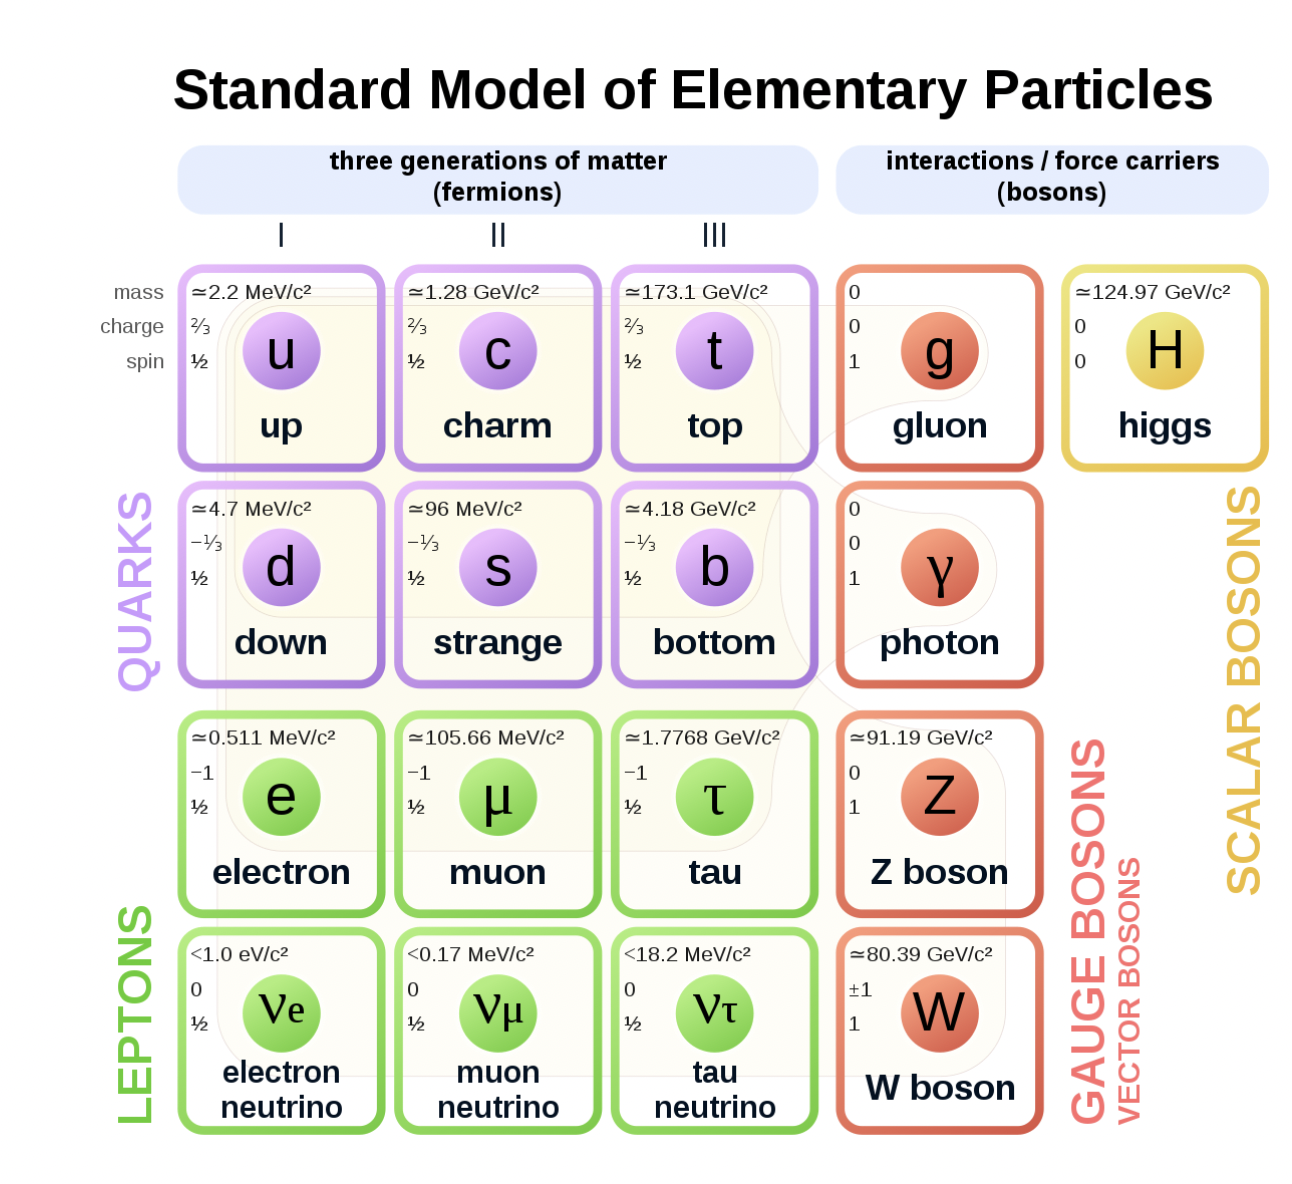
\includegraphics[scale=0.7]{fig/CreativeCommonsSM.png}
    \caption{The Fundamental Particles of the Standard Model of Particle Physics.}
    \label{fig:SMTable}
\end{figure}

\begin{figure}
    \centering
    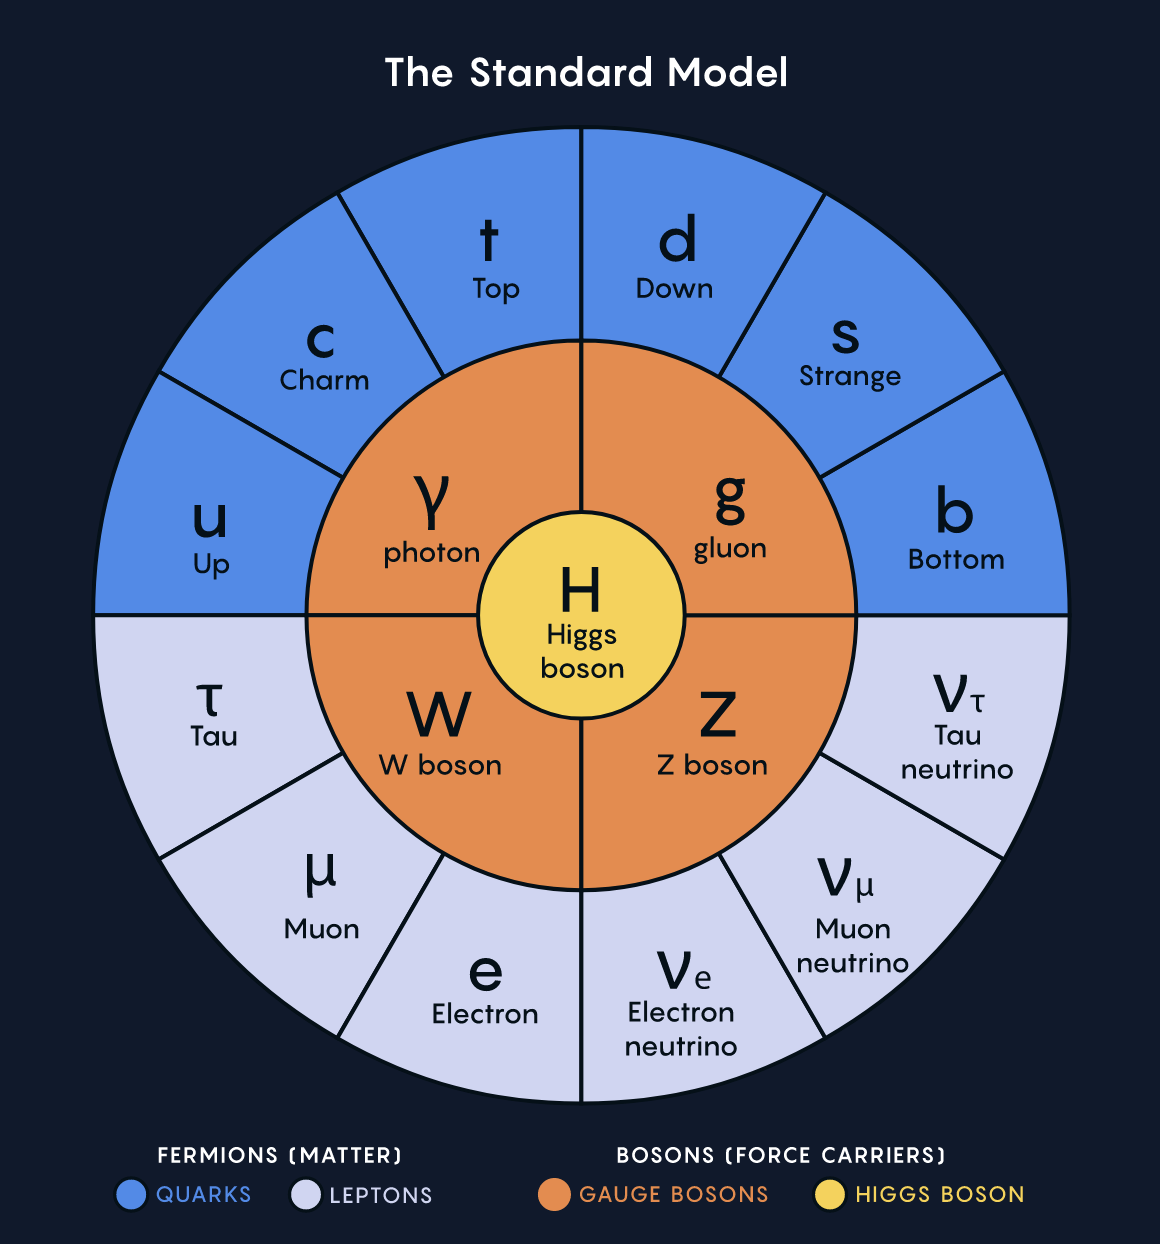
\includegraphics[scale=0.7]{fig/SM.png}
    \caption{The Standard Model of Particle Physics depicting the central role of the Higgs Boson~\cite{QuantaMagNewMap}.}
    \label{fig:SMDiagram}
\end{figure}


% \subsection{Rules of Interaction} 

% \begin{figure}[!htbp]
% 	\centering
% % 	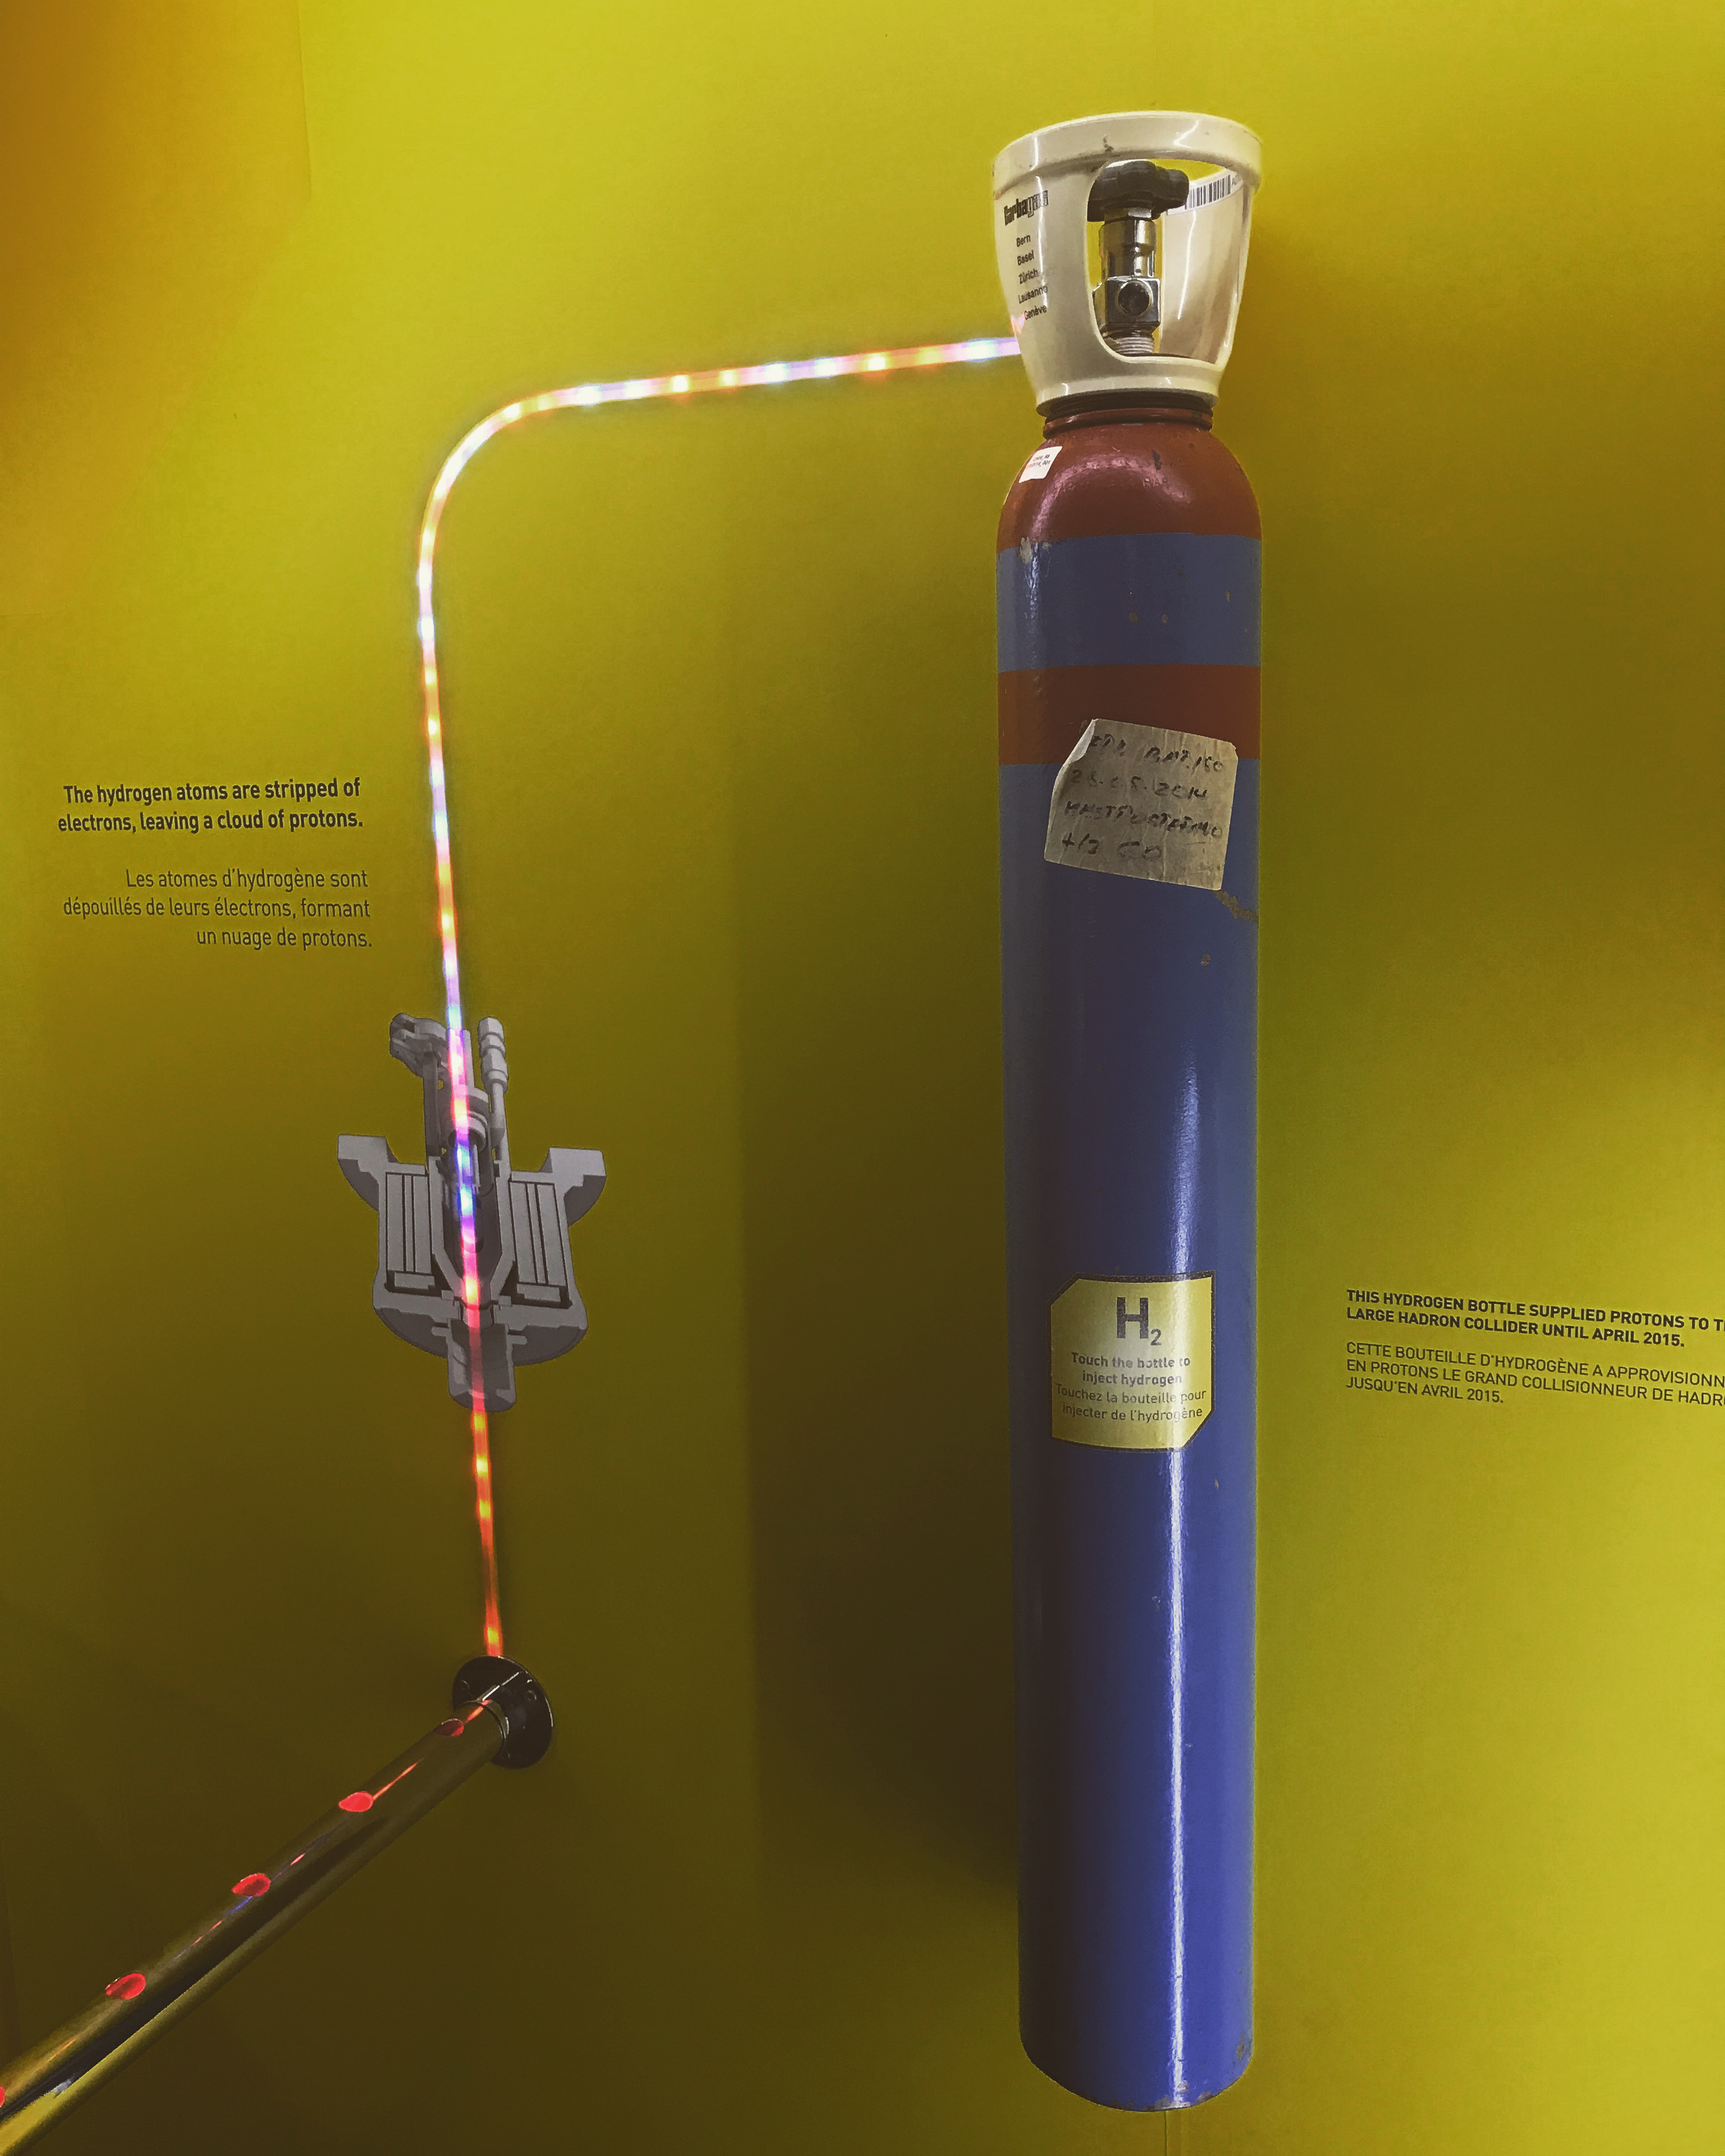
\includegraphics[scale=0.038]{fig/H2Bottle.JPG}
%     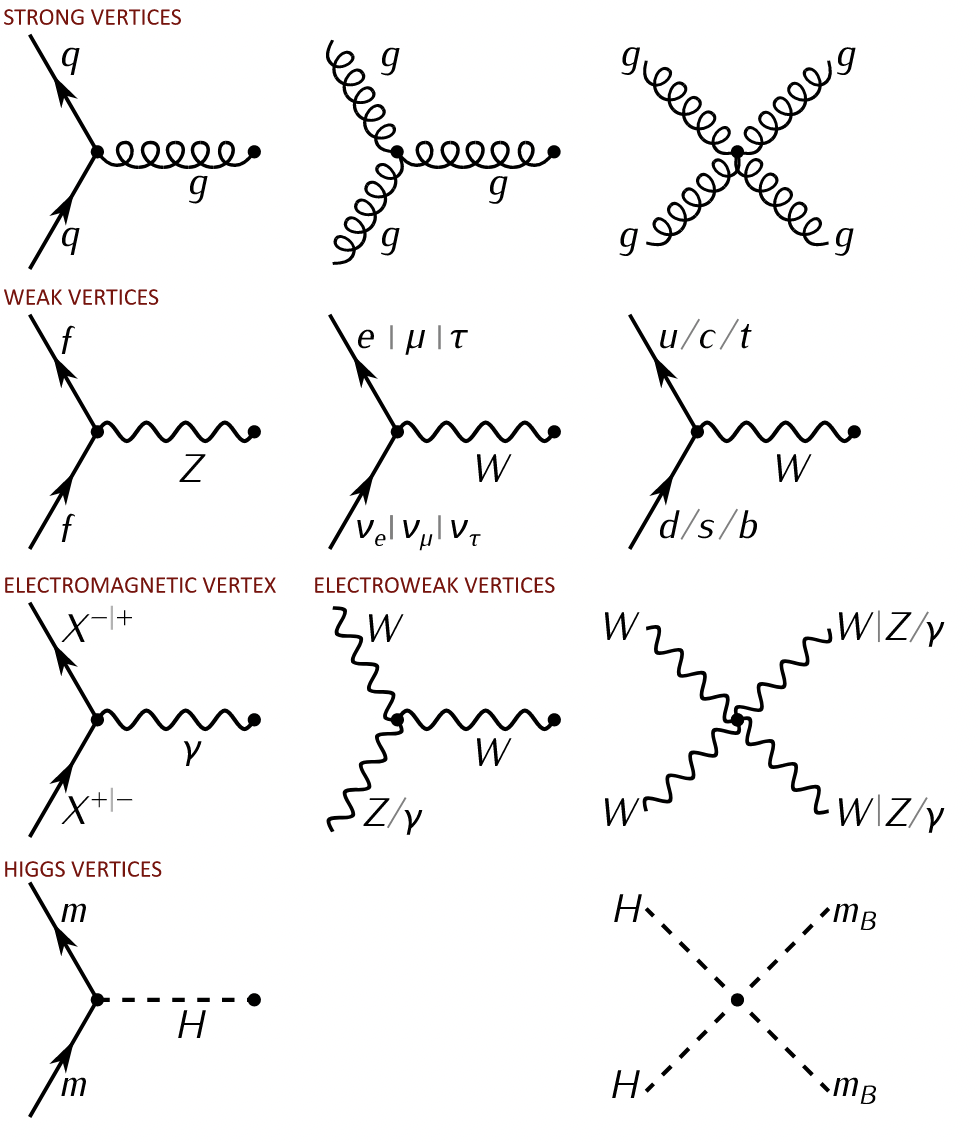
\includegraphics[scale=0.6]{fig/StandardModelOfParticlePhysics.png}
% 	\caption{Fundamental Vertices of the Standard Model. These Feynman diagrams represent the interactions between the fermions and vector gauge bosons in the SM. The W boson charge is determined by the charge of the fermions they interact with and the interaction has to observe the conservation of electric charge.}
% 	\label{fig:FundamentalVertices}
% \end{figure}

% Particle interactions are described intuitively by Feynman diagrams. These Feynman diagrams serve as mathematical book keeping aids which enable physicists to predict the outcomes of particle collision experiments and particle behaviour within the framework of QFT. Each line in a diagram corresponds to a specific particle while the vertices represent the interactions between these particles.

\subsection{QED: Electromagnetic Interaction}

QED or Quantum Electrodynamics is a quantum field theory component of the Standard Model that merges the principles of quantum mechanics with electrodynamics. QED at its core describes the interactions between electrically charged particles via photon exchange and it is described by a basic QED vertex shown in Fig.~\ref{fig:QEDVertex}. 

\begin{figure}[!htbp]
    \label{fig:QEDVertex}
	\centering
    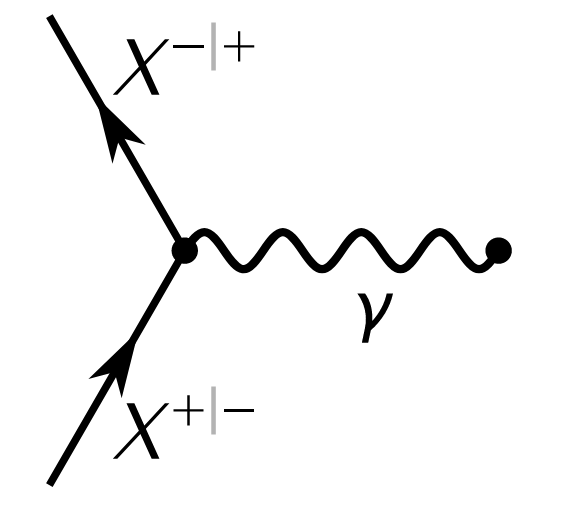
\includegraphics[scale=0.6]{fig/QEDfudnamental.png}
	\caption{QED Feynman diagram basic vertex showing an interaction between a fermion and an anti-fermion emitting a photon.}
\end{figure}

The fundamental principle of QED revolves around the preservation of electric charge which implies a U(1) symmetry. It is also an example of an abelian gauge theory which is a type of QFT where the gauge transformations commute. 

% The rules of interaction of particles are dictated by symmetry rules governed by the concepts of local and global gauge invariance. From the Lagrangian, $~\mathcal{L}$ the participating quantum fields must obey certain symmetries where the $~\mathcal{L}$ remains invariant under an arbitrary gauge transformation. To illustrate this 

We consider the Lagrangian density of a free Dirac field, $\mathcal{L}_D$ given by:

\begin{equation}
\label{eq:DiracLag}
    \mathcal{L}_{\text{Dirac}} = \bar{\psi}(i\gamma^\mu\partial_\mu - m)\psi. 
\end{equation}

Here, $\gamma^\mu$ are the Dirac matrices, and $\psi$ are the spin-1/2 fields. This Lagrangian has a global $U(1)$ Abelian symmetry, s.t. it remains invariant under this transformation,

\begin{equation}
\label{eq:U1global}
    \psi(x) \rightarrow e^{i\alpha} \psi(x).
\end{equation}

A local transformation on the other hand, where $\alpha$ is replaced with $\alpha(x)$, requires a change in the derivative $\partial_u$ with the covariant derivative defined by
\begin{equation}
\label{eq:CovariantDerivative}
    D_{\mu}  = (\partial_{\mu} - ig A_{\mu}) , 
\end{equation}

where $\partial_{\mu}$ is the partial derivative with respect to the spacetime coordinate $x^{\mu}$, $g$ is the coupling constant, and $A_{\mu}$ is the gauge field. Substituting Eq.~\ref{eq:CovariantDerivative} into Eq.~\ref{eq:DiracLag}, we get a resultant Lagrangian that is invariant under the 

\begin{equation}
\label{eq:AuGaugeTransformation}
   A'_{\mu} = A_{\mu} - \frac{1}{g} \partial_{\mu} \alpha(x), 
\end{equation}

and the local transformation in eq.~\ref{eq:U1global}. Here $A_\mu$ is referred to as the photon field. These steps could be extended to non-Abelian symmetries, where transformation operators do not commute, whose treatment is explained in more detail in standard gauge theory texts such as Ref~\cite{Peskin:1995ev}.

The expression for the QED Lagrangian Density is as follows:

\begin{equation}
\label{eq:QEDLagrangian}
\mathcal{L}_{\textnormal{QED}} = \bar{\psi} (i \gamma^{\mu} \partial_{\mu} - m) \psi - \frac{1}{4} F_{\mu\nu} F^{\mu\nu} - Q \bar{\psi} \gamma^{\mu} \psi A_{\mu},
\end{equation}

where $\psi$ is a fermion field and Q is the electric charge. Each term of the Lagrangian can be understood as the Dirac Lagrangian~\ref{eq:DiracLag} plus the Maxwell's terms plus the fermion field and photon field interaction. This new covariant derivative introduces $A_{u}$ as a new vector field which we we will see as follows is nothing but the electromagnetic four vector potential. Both $A_\mu$ and $D_\mu$ must be invariant under the $U(1)$ transformation as in Eq.~\ref{eq:U1global} and it follows that the commutator of the covariant derivative is also invariant under the same transformation. Expanding the commutator, we find that we can rewrite it in terms of the Electromagnetic field tensor $F^{\mu\nu}$:

\begin{equation}
\begin{align*}
        \label{eq:QEDcommutator}
    [D_\mu, D_\nu] &= iQ(\partial_\mu A_\nu + A_\mu \partial_\nu - \partial_\nu A_\mu - A_\nu \partial_\mu) \\
    &= iQ(\partial_\mu A_\nu - \partial_\nu A_\mu) \\ &= iQ$F^{\mu\nu}$ .
\end{align*}
\end{equation}

We can now write $\mathcal{L}_{QED}$ in the gauge invariant form by substituting the partial derivative with the covariant derivative in Eq.~\ref{eq:CovariantDerivative}.  The QED Lagrangian can be recast simply as:

\begin{equation}
\label{eq:QEDLagrangian}
\mathcal{L}_{\textnormal{QED}} = \bar{\psi} (i \gamma^{\mu} D_{\mu} - m) \psi - \frac{1}{4} F_{\mu\nu} F^{\mu\nu},
\end{equation}

\subsection{QCD: Strong Interactions}

\begin{figure}[!htbp]
	\centering
    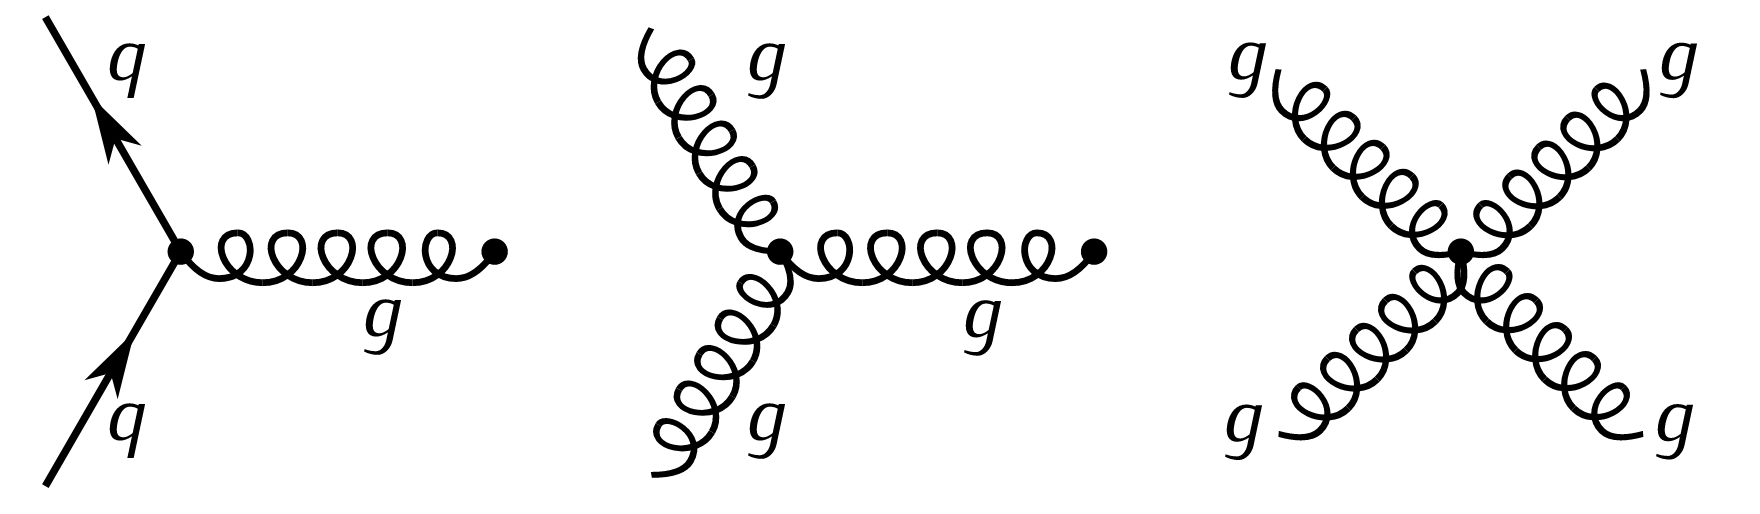
\includegraphics[scale=0.4]{fig/QCDFundamentalVertices.png}
	\caption{QCD Fundamental vertices where quark-gluon interactions (left) and gluon self-interactions (middle and right) are shown.}
	\label{fig:QCDFundamentalVertices}
\end{figure}

Quantum Chromodynamics (QCD) is the segment within the framework of the Standard model that explains the dynamics of interactions between color-charged particles namely quarks and gluons. This is mathematically captured through transformations within the SU(3) symmetry group to which three distinct charge quantum numbers, namely red, green, and blue are introduced. This stands in stark contrast to QED, which involves a single electric charge. Initial experiments unveiled a crucial aspect of the quantum field theory governing quark interactions - the strength of the interactions decreases as the momentum of the interacting particles escalates. This behaviour is a hallmark of non-Abelian gauge theories of which QCD belongs to. 

The mathematical structure of quantum chromodynamics can be treated as an extension of the idea of local gauge invariance in QED, where the $U(1)$ gauge group as in Eq.~\ref{eq:U1global} is replaced by the $SU(3)$ group of phase transformations on the quark color field: 

\begin{equation}
    \label{eq:QCDgaugeinv}
    q \rightarrow e^{ig_sT^{a}}q,
\end{equation}

where $q$ is the quark field, and $g_s$ is the strong coupling constant. 

QCD is a non-abelian gauge theory due to the non-commutative generators within this group. The generators of the SU(3) group are as follows:

\begin{equation}
    \label{eq:QCDGenerators}
    [T^a, T^b] = if^{abc} T^c
\end{equation}

where $T^{a} = \lambda^{a}/2$, $\lambda^{a}$ are the Gell-Mann matrices and $f^{abc}$ are the structure constants which are antisymmetric coefficients that govern the commutation relations between the Gell-Mann matrices describing how gluons, the force carriers of the strong interaction, interact with each other via the color charges of quarks. The Gell-Mann matrices consist of a collection of eight 3x3 matrices that are Hermitian and have a trace of zero. 

In a similar vein as in Eq.~\ref{eq:AuGaugeTransformation}, we need to introduce the eight gauge fields $G^{a}_{\mu}$, each transforming as:

\begin{equation}
    \label{eq:QCDGauge}
    G^{a}_{\mu} \rightarrow G^{a}_{\mu}' - \frac{1}{g}\partial_{\mu} \alpha_a
\end{equation}

From this we can form a covariant derivative, 
\begin{equation}
    \label{eq:CovariantDerivativeQCD}
    D_\mu = \partial_\mu + igT^{a}G^{a}_\mu.
\end{equation}

This introduces 8 gluon fields, $G^{a}_{u}$, each corresponding to permissible color combinations within the group. Plugging this in the free Lagrangian akin to the Dirac Lagrangian in Eq.~\ref{eq:DiracLag},

\begin{equation}
    \label{eq:FreeLag}
    \mathcal{L} = \bar{q}_{j}(i\gamma^{\mu} \partial_{\mu} - m)q_j, 
\end{equation}

where $q_i$, $i = 1,2,3$ denote the three color fields. The QCD analogue of Eq.~\ref{eq:QEDLagrangian} then becomes, 
\begin{equation}
    \label{eq:FreeLag}
  \mathcal{L} = \bar{q}(i\gamma^{\mu} \partial_{\mu} - m)q - g(\bar{q}\gamma^{\mu}T_{\alpha}q)G^{a}_{\mu}. 
\end{equation}

This is however still not a fully gauge invariant Lagrangian as the last term transformation, since we already from Eq.~\ref{eq:QCDGenerators} that the Gell-Mann matrices don't commute. To mitigate this problem an extra term must be added to Eq.~\ref{eq:QCDGauge}, 

\begin{equation}
    \label{eq:QCDGaugeCorrected}
    G^{a}_{\mu} \rightarrow G^{a}_{\mu} - \frac{1}{g}\partial_{\mu} \alpha_a -f_{abc}\alpha_{b}-G^{a}_{\mu}.
\end{equation}

We then have the final gauge invariant QCD of the form:

\begin{equation}
    \label{eq:QCDLag}
  \mathcal{L} = \bar{q}(i\gamma^{\mu} \partial_{\mu} - m)q - g(\bar{q}\gamma^{\mu}T_{\alpha}q)G^{a}_{\mu} - \frac{1}{4}G^{a}_{\mu\nu}G^{\mu\nu}_{a},
\end{equation}

or in terms of the covariant derivative, 

\begin{equation}
    \label{eq:QCDLag}
  \mathcal{L}_{\textnormal{QCD}} = \bar{q}i\gamma^{\mu} D_{\mu}q - \frac{1}{4}G^{a}_{\mu\nu}G^{\mu\nu}_{a},
\end{equation}

Gluons can directly partake in interactions involving their own color properties. One can expand the QCD Lagrangian~\ref{eq:QCDLag} in terms of the transformation in Eq.~\ref{eq:QCDGaugeCorrected}, and write in symbolic form in terms of increasing orders of ``G"~\cite{Halzen:1984mc},

\begin{equation}
    \label{eq:QCDSymbolic}
  \mathcal{L}_{\textnormal{QCD}} = ``\bar{q}q" + ``G^2" + g``\bar{q}{q}G" + g``G^{3}" + g^2``G^{4}".
\end{equation}

The first two terms describe the free propagation of quarks and gluons. The last three terms are represented schematically in Fig.~\ref{fig:QCDFundamentalVertices}. The first vertex illustrates the interaction between quarks and gluons, while the subsequent two shows 3- and 4-point self-interactions of gluons. 

Gluons' ability to self-interact directly in Quantum Chromodynamics (QCD) results in a significant QCD feature: the strengthening of the coupling between quarks with increasing distance. This phenomenon leads to the preferred formation of new quark-antiquark pairs from the vacuum when attempting to separate bound quarks, causing the creation of two mesons instead of isolated quarks. This confinement of quarks, known as confinement, prohibits the observation of bare quarks in nature, allowing only color-neutral QCD states. Consequences of confinement are evident at high-energy colliders, where high-energy quark or gluon generation results in chains of hadrons forming hadronic jets through fragmentation or hadronization. These jets are pivotal signatures in particle detectors like CMS. At lower energies, scattering interactions lack the energy for jet formation, yielding a spread of hadrons, prevalent in background processes at colliders like the LHC. The top quark, with a short lifetime, decays weakly, sidestepping hadronization, making it a study candidate for ``bare" quarks. Confinement introduces computational challenges, particularly in the non-perturbative QCD regime below the confinement scale, where interaction predictions rely on heuristic tools. Above this scale, asymptotic freedom manifests, with quarks acting as free particles at high energies, valid for hard scattering interactions at colliders through perturbation theory.

\subsection{Electroweak Interactions}

The final piece of the SM, the weak interactions, is an extension of QED which describes how particles charged under weak isospin interact with the $W^{\pm}$ and Z bosons. QED was initially developed to describe the interactions of electrically charged fermions. Following spontaneous symmetry breaking, the photon gains the ability to interact with the electrically charged $W^{\pm}$ bosons as well. Additionally, QED on its own, can function independently as a renormalizable, Abelian gauge theory. However the weak interaction involving the $W^{\pm}$ and Z bosons cannot be adequately described by a standalone gauge theory. It has been determined that these three weak interaction vector bosons and the massless photon in QED need to be collectively addressed within the framework of an $SU(2) \times U(1)$ symmetry in order to explain the observed weak force in the natural world. 

The electroweak theory  has  $SU(2) \times U(1)$ gauge group which have the following fundamental fields: $W^1_{\mu}, W^2_{\mu}, W^3_{\mu}$, associated with the three generators of $SU(2)_{L}$ and $B_{\mu}$, associated with $U(1)_{Y}$. The force mediators, $W^{\pm}$, Z and $\gamma$ are orthogonal combinations of these fundamental fields, which we will show later.

As $SU(2)$ is also a non-Abelian theory, so the weak gauge bosons endowed with charges related to weak isospin, like how gluons bear color charges in QCD. Consequently, they exhibit self-interactions including cubic and quartic couplings of the form $WW\gamma$, $W W Z$, $W W W W$, $W W \gamma\gamma$, $W W ZZ$, and $W W Z\gamma$. The mixing among the original states of $SU(2) \times U(1)$ leads to distinct outcomes that distinguishes the electroweak sector with QCD, the other non-Abelian theory. These unique consequences are essential for aligning theoretical predictions with experimental observations. The theory is also chiral in nature and parity-violating  \cite{Kobayashi:1973fv}., i.e. the symmetry transformations act on ``left-handed" and ``right-handed" fermion fields differently each. This property that the W-boson only couples to fermions of left-handed chirality is a crucial property of the SM and is encoded in the V-A theory\cite{ParticleDataGroup:2018ovx} to explain the the weak nuclear force, which is responsible for processes such as beta decay in atomic nuclei. It is responsible for many of the surprising features of the weak interactions, both the most attractive and the most puzzling ones. 

\begin{figure}[!htbp]
	\centering
% 	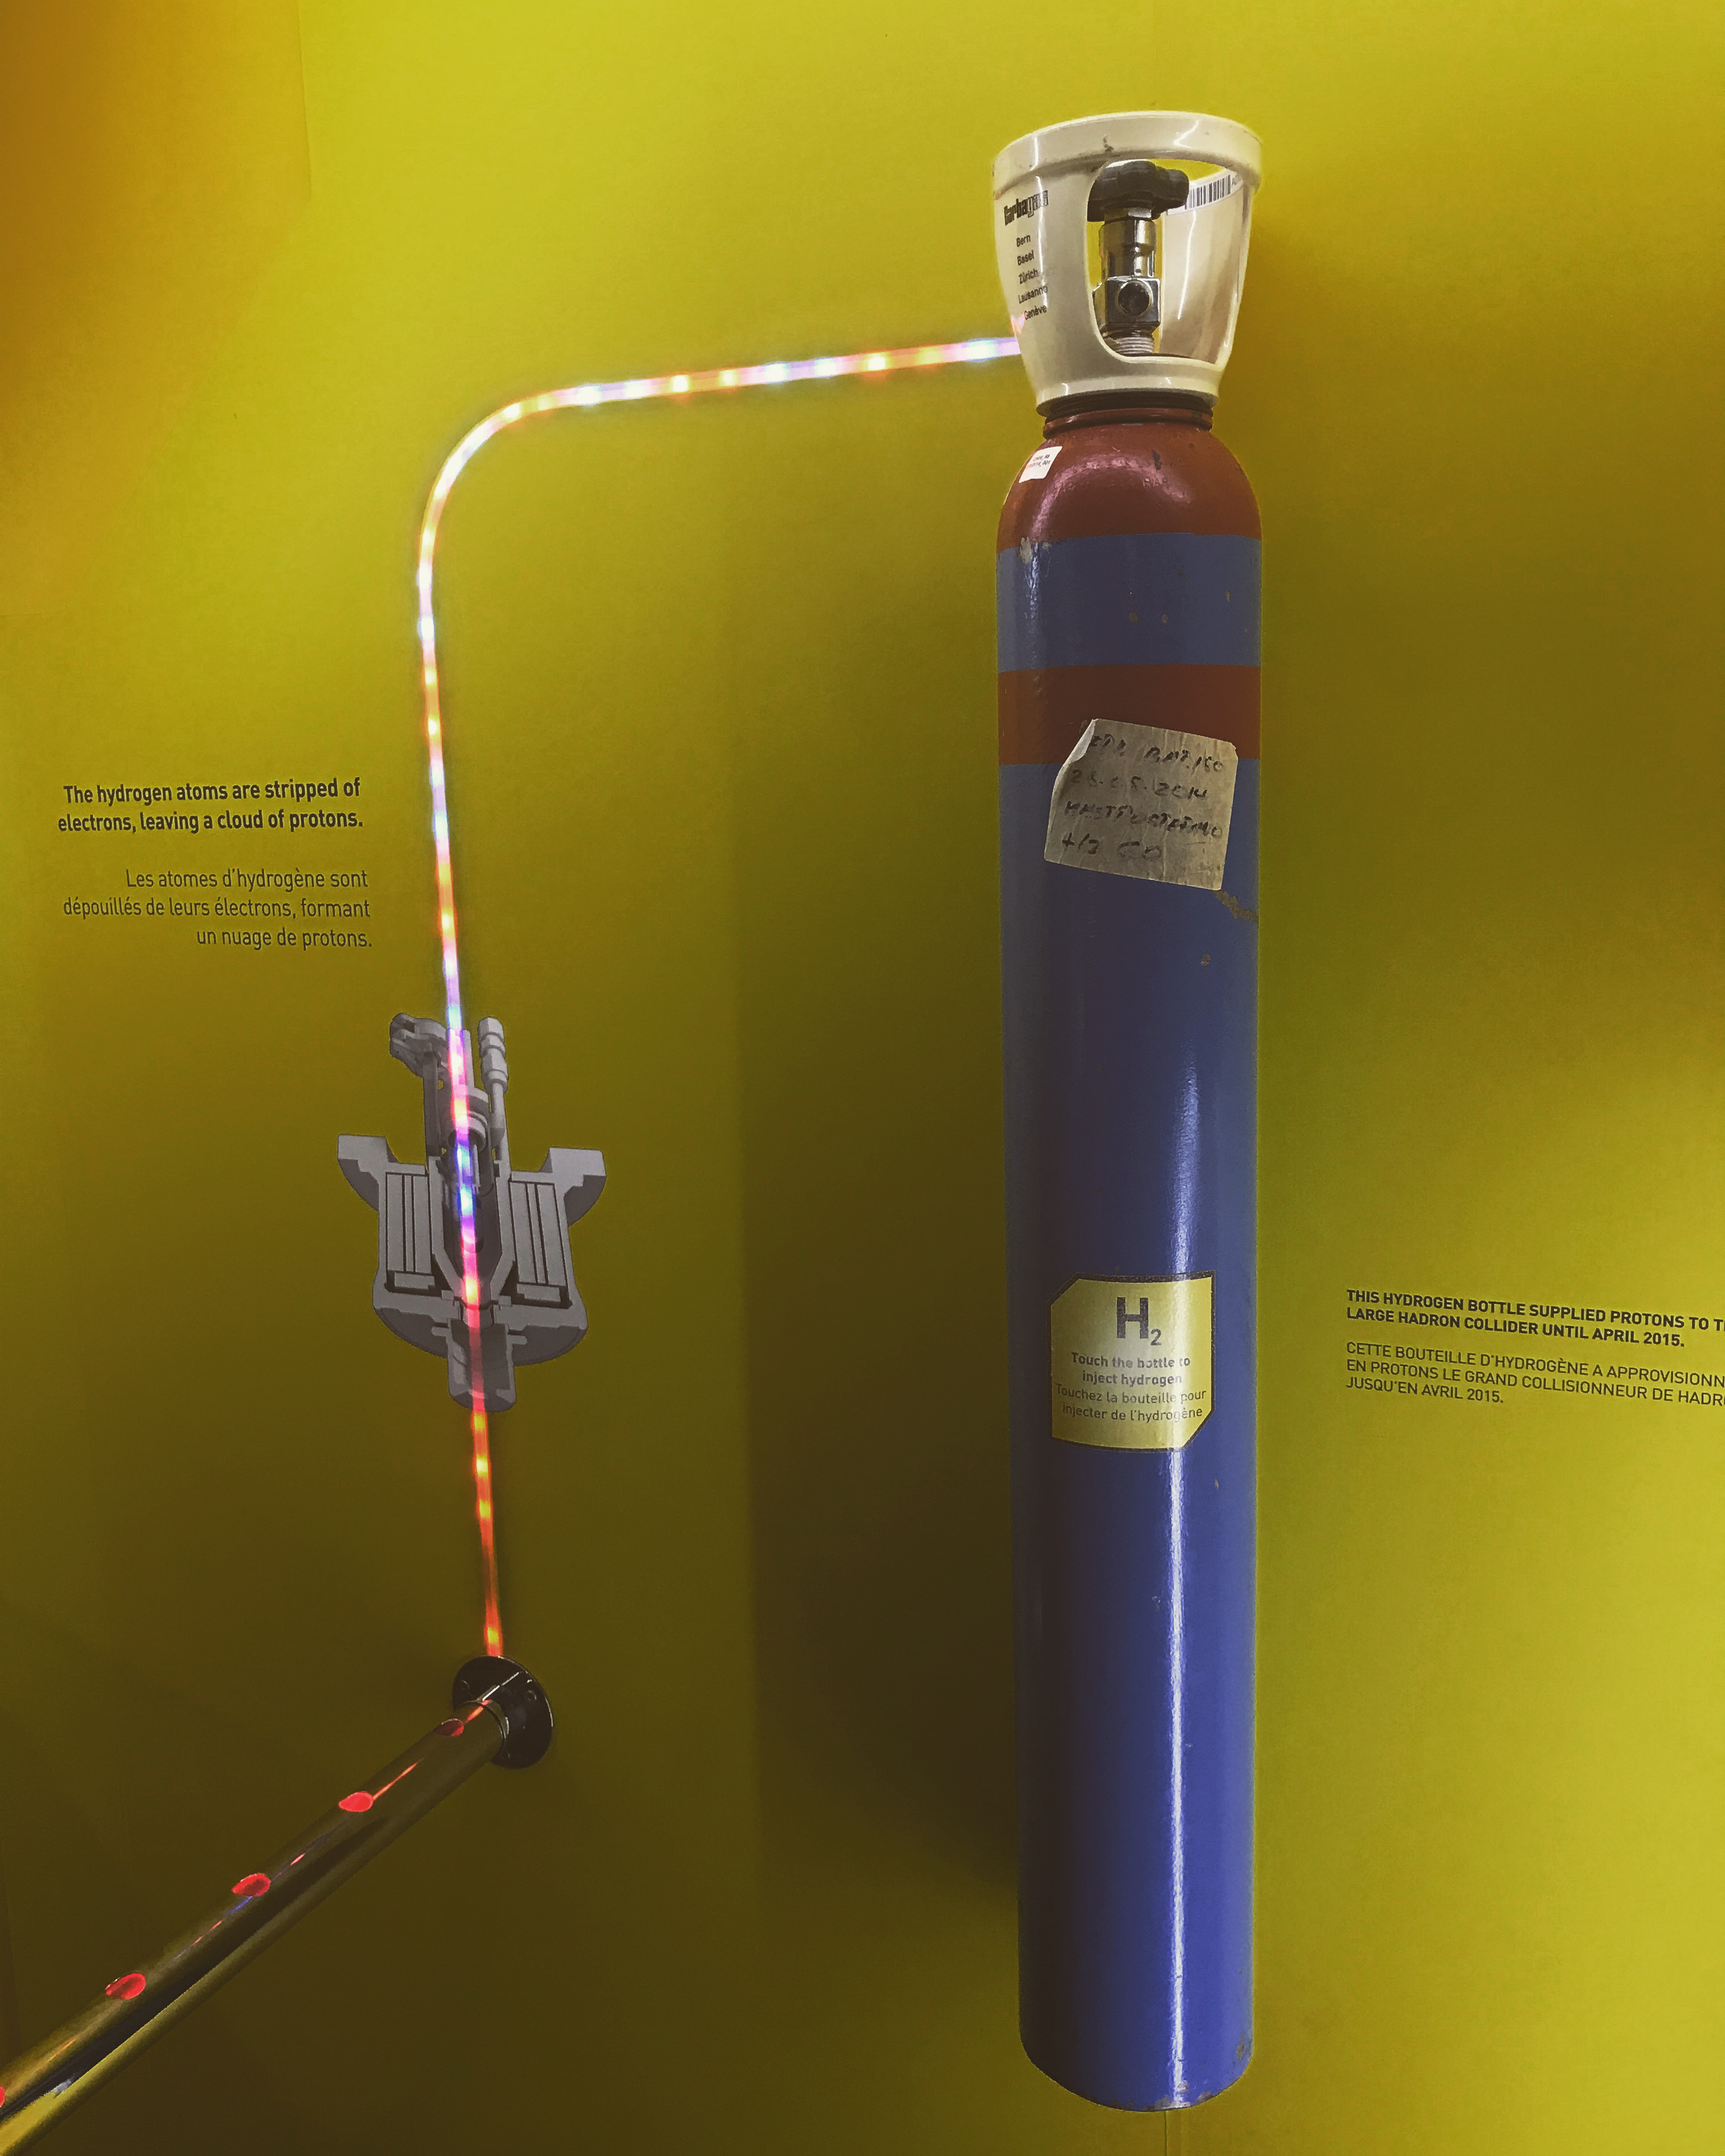
\includegraphics[scale=0.038]{fig/H2Bottle.JPG}
    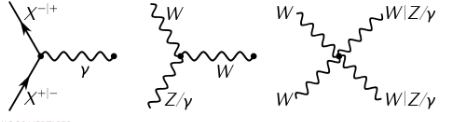
\includegraphics[scale=1.0]{fig/ElectroweakVertices.png}
	\caption{Electroweak Interaction Vertices. X are fermions.}
	\label{fig:Electroweak}
\end{figure}

The mathematical formalism of the electroweak interactions extension of the QED/QCD formalism. To include weak interactions we must write the covariant derivative as:

\begin{equation}
    \label{eq:CovariantDerivativeElectroWeak}
    D_\mu = \partial_\mu - ig_wT^{i}W_{\mu}^{i} - ig_{em}YB_{\mu}, 
\end{equation}

where the operators $T_{i}$ and $\textbf{Y}$ are the generators of the $SU(2)_{L}$ and $U(1)_{Y}$ groups of gauge transformations, respectively. These generators satisfy 

\begin{equation}
    \label{eq:ConservationElectroweakQNum}
   Q = T^3 + \frac{Y}{2}.
\end{equation}
The eigenvalues of these generators, T and Y are also known as the weak isospin and the weak hypercharge quantum numbers. This follows that the electromagnetic current is a combination of the neutral currents and we can write:


\begin{equation}
    \label{eq:ConservationElectroweakCurrent}
   j^{em}_{\mu}= J^3_{\mu} + \frac{1}{2}j^{Y}_{\mu}.
\end{equation}

For the interaction lagrangian, we recall from QED that the interaction is mediated by gauge fields as:

\begin{equation} 
\label{eq:QEDint}
L^{int}_{QED} = -iej^{em}_{\mu} A_{\mu}
\end{equation}

where $j^{em}_{\mu} = \bar{\psi}\gamma^\mu\psi
$ is the $U(1)_{em}$ current and $A_{\mu}$ is the gauge field photon. We copy this for the case of the EW interaction lagrangian and write it in terms of current triplets and singlets

\begin{equation} 
\label{eq:QEDint}
\mathcal{L}^{int}_{EW} = -igj^{i}_{\mu} W^{i\mu} - \frac{ig'}{2} j^{Y}_{\mu} Y^\mu B_\mu
\end{equation}

where the SU(2) part can be expanded as:

\begin{equation} 
\label{eq:SU(2)current}
-igj^{i}_{\mu} W^{i\mu} = -ig\bar{\chi}_L\gamma_{\mu}T\cdotW^{\mu}\chi_{L}
\end{equation}

\begin{equation} 
\label{eq:U(1)}
\frac{ig'}{2} j^{Y}_{\mu} Y^\mu B_\mu = -ig'\bar{\psi}\gamma_{\mu}\frac{Y}{2} \psiB^{\mu}. 
\end{equation}

The vector bosons associated with the particles $W^{\pm}$, Z and $\gamma$, can be constructed as linear combinations of $W^{i}_{\mu}$ gauge field triplet and the singlet $B^{\mu}$. The massive vector boson is written as,

\begin{equation} 
\label{eq:MassiveVecBoson}
W^{\pm\mu} = \frac{1}{\sqrt{2}}(W^{1}_{\mu} \mp iW^{2}_{\mu}).
\end{equation}
The neutral vector bosons $A_{\mu}$ and $Z^{\mu}$ associated with the massless photon and and massive $Z^{0}$ boson are written as follows:

\begin{equation} 
\label{eq:NeutralVectorBosons}
\begin{align*} 
A^{\mu} = B^{\mu}\cos\theta_{w} + W^{3\mu} \sin\theta_{w} ,\\ 
Z^{\mu} = -B^{\mu}\sin\theta_{w} + W^{3\mu} \cos\theta_{w}.
\end{align*}
\end{equation}

Here $\theta_w$ is the ``weak mixing" or ``Weinberg" angle. Substituting the Eqs.~\ref{eq:NeutralVectorBosons} to the electroweak interaction Lagrangian, grouping together terms with $A^{\mu}$ and $Z^{\mu}$\cite{Halzen:1984mc} and using Eq.~\ref{eq:ConservationElectroweakCurrent}, we find that $\theta_w$ can be written as 

\begin{equation} 
\label{eq:weinbergAngle}
e = g\sin\theta_{w} = g'\cos\theta_{w}.
\end{equation}

In practice, $e$, which is the electron charge and $\sin\theta_{w}$ are used as parameters for the standard model to be measured experimentally. Found in the second term with $Z^{\mu}$ is the weak neutral current:
\begin{equation} 
\label{eq:neutralcurrent}
J^{NC}_{\mu} = \frac{g}{\cos\theta_{w}} (j^3_{u} - sin^2\theta_w j^{em}_{\mu}).
\end{equation}


Here we highlight some key aspects of weak interactions. Firstly, we discuss flavor mixing, which is prominent in quarks but absent in leptons. Weak interactions uphold lepton generation conservation, preventing mixing between different lepton generations. For instance, a W boson interacts with an electron and an electron neutrino but not with a muon and an electron neutrino~\cite{MarkusKluteLectures}. 

% Here we highlight a few important things for the weak interactions. First, is the flavor mixing of quarks which does not occur in leptons. The weak interactions respect the lepton generation, such that there is no mixing between generations. A W boson couples to an electron and an electron neutrino, but not to a muon and an electron neutrino

\begin{equation} 
\begin{align*}
\label{eq:CKMMatrix}
        \begin{pmatrix}
        \nu_e \\
        e 
    \end{pmatrix}, 
    \begin{pmatrix}
         \nu_\mu \\
         \mu \\
    \end{pmatrix},
     \begin{pmatrix}
        \nu_\tau \\
        \tau \\
    \end{pmatrix}
\end{align*}
\end{equation}

In contrast, quark generation is not conserved. Instead, we have the quark doublets that participate in the $SU(2)$ symmetry of the charged-current weak interaction are defined as follows:

\begin{equation} 
\begin{align*}
\label{eq:CKMMatrix}
        \begin{pmatrix}
        u \\
        d' 
    \end{pmatrix}, 
    \begin{pmatrix}
         c \\
         s' \\
    \end{pmatrix},
     \begin{pmatrix}
        t \\
        b' \\
    \end{pmatrix}
\end{align*}
\end{equation}

The primed coordinates are given by the relation involving the CKM matrix in Eq.~\ref{eq:CKMMatrix}. This flavor state mixing, non-conservation in the case of quarks is captured in the CKM matrix, denoted as V: 

\begin{equation} 
\begin{align*}
\label{eq:CKMMatrix}
        \begin{pmatrix}
        d' \\
        s' \\
        b' \\
    \end{pmatrix} &=
    \begin{pmatrix}
         V_{ud} & V_{us} & V_{ub} \\
         V_{cd} & V_{cs} & V_{cb} \\
         V_{td} & V_{ts} & V_{tb}
    \end{pmatrix}
     \begin{pmatrix}
        d \\
        s \\
        b \\
    \end{pmatrix}
\end{align*}
\end{equation}

In this matrix, the elements $V_{ij}$ represent the complex numbers that describe the mixing between different quark flavor states. The indices (i, j) correspond to the initial and final quark flavor states, where "u" stands for up quark, "d" for down quark, "s" for strange quark, "c" for charm quark, "t" for top quark, and "b" for bottom quark. Since this matrix is mostly diagonal, it results in the suppression of couplings between an up-type quark from one generation and a down-type quark from another to the W boson. In the original Standard Model, neutrinos were considered massless, and thus, there was no mixing in the leptonic sector. However, as we now know that neutrinos have mass, one way to account for this is by introducing right-chiral singlets for neutrinos, allowing them to acquire mass in a manner similar to other Standard Model fermions. This introduces a mixing matrix in the leptonic sector known as the PMNS matrix \cite{Maki:1962mu}. 

Historically, the masses of the weak force carriers had been a significant puzzle. The SM of the 1970s or also known as Glashow-Salam-Weinberg theory predicted the existence of the W and Z bosons but did not provide exact predictions of their masses. They were measured later at CERN with the UA1 experiment (W) and the UA2 collaboration (Z-boson). The origin of their masses was elusive and couldn't be incorporated back then into the SM theory in a gauge-invariant matter. This posed as a challenge for achieving true unification. We will see in the next section the significance of the Higgs Mechanism in how particles acquire mass through spontaneous symmetry breaking and preserving the gauge invariance of the theory.



% In contrast, in theories with unbroken symmetries like Quantum Electrodynamics (QED) and Quantum Chromodynamics (QCD), gauge bosons are massless. 
% However, mass terms can be introduced in a gauge-invariant manner when symmetries are broken. Therefore, the symmetry associated with the weak force mediators must indeed be a broken symmetry. The Higgs Mechanism effectively breaks the symmetry of the electroweak $SU(2) \times U(1)$ group while demonstrating how the inclusion of a scalar field preserves the gauge invariance of the theory.

\subsection{Higgs Mechanism and Spontaneous Symmetry Breaking} \label{sec:HiggsMechanism}

The Higgs mechanism was conceived originally to provide mass to the weak gauge bosons. However, it also offers a means of imparting mass to fermions through the Yukawa coupling. We will show both in this section. Consequently, the Higgs boson forms direct connections with all massive particles within the Standard Model. Furthermore, the Higgs boson itself possesses mass, though it is not a gauge boson. It acquires a mechanism for self-interaction through the Higgs potential. The interaction vertices involving the Higgs are illustrated in Figure~\ref{fig:HiggsVertices}. The first of these (Figure 3.6a) delineates the interaction between the Higgs boson and massive particles. 

\begin{figure}[!htbp]
	\centering
     \label{fig:HiggsVertices}
    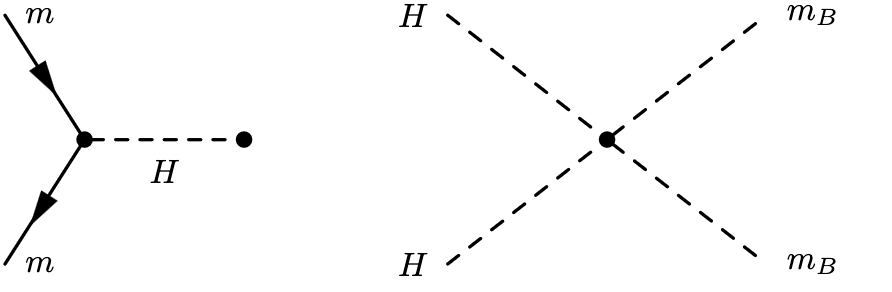
\includegraphics[scale=1.0]{fig/HiggsInteraction.png}
	\caption{Higgs Interaction Vertices.}
\end{figure}

An ad hoc introduction of vector boson mass terms in the Lagrangian leads to a violation of gauge invariance. For the QED Lagrangian in Eq.~\ref{eq:QEDLagrangian}, a mass term of the form 

\begin{equation}
    \label{eq:AmuWrongMassterm}
    \mathcal{L} = \frac{1}{2}M^2_{A}A^{\mu}A_{\mu}
\end{equation}

would destroy gauge invariance under the transformation of $A_{\mu}$(Eq.~\ref{eq:AuGaugeTransformation}). To generate mass for the gauge bosons, the local gauge symmetries must be broken. 

Standard introductory particle physics texts and lectures~\cite{Halzen:1984mc}
usually begin with a toy model where a single complex scalar field is coupled to the U(1) gauge field 

\begin{equation}
    \label{eq:ToyScalarFieldLagrangian}
    \mathcal{L} = -\frac{1}{4} F_{\mu\nu}F^{\mu\nu} + |D_{\mu}|^2 - V(\phi)
\end{equation}

% (\partial_{\mu}\phi)(\partial^{\mu}\phi) - \frac{1}{2} \mu^2 |\phi|^2 - \lambda |\phi|^4

where $D_\mu = \partial_{\mu} - ieA{\mu}$ and $V =\mu^2 |\phi|^2 - \lambda |\phi|^4 $. For $\mu^2 < 0$, this is just the QED Lagrangian for a charged complex scalar particle of mass $\mu$ save for the $\phi^4$ self-interaction term. It has a unique minimum at zero and does not break the symmetry. To generate the mass terms we take $\mu^2 > 0$. This breaks the $U(1)$ symmetry and has a minimum at 

\begin{equation}
    \label{eq:Minimum}
    <\phi> = \frac{v}{\sqrt{2}} = \sqrt{-\frac{\mu^2}{2\lambda}}.
\end{equation}
This is a circle of minimum with radius $v$ and is shown in Fig.~\ref{fig:MexicanHat}. 

For convenience we can rewrite $\phi$ in terms of real fields, 

\begin{equation}
    \label{eq:RealFields}
    \phi = \frac{v+h}{\sqrt{2}}e^{i\frac{\theta}{v}},
\end{equation}

here $h$ and $\chi$ are the Higgs and Goldstone bosons respectively

\begin{align}
\label{eq:HiggsGoldstone}
    L = &-\frac{1}{4} F_{\mu\nu} F^{\mu\nu} - e v A_\mu \partial^\mu \chi + \frac{e^2 v^2}{2} A_\mu A^\mu \nonumber \\
    &+ \frac{1}{2} (\partial_\mu h \partial^\mu h - 2\mu^2 h^2) \nonumber \\
    &+ \frac{1}{2} \partial_\mu \chi \partial^\mu \chi + \textnormal{interaction terms}. \label{eq:HiggsGoldstone}
\end{align}


With this new Lagrangian, the photon is imparted a mass $m_A = ev$. The theory now has a Higgs boson $h$ of mass $m_h = \sqrt{2\mu} =\sqrt{2\lambda v^2} \lambdav$, and a massless Goldstone $\theta$. If we choose the following gauge transformation:

\begin{equation}
\label{eq:GoldstoneGauge}
A_{\mu} \rightarrow A_{\mu} + \frac{1}{ev}\partial_{\mu}\theta
\end{equation}

the theory will be independent of $\theta$. The theory will not just have two interacting massive particles which are $A_\mu$ and $h$. 

The procedure could be generalized for an $SU(n)$ gauge symmetry~\cite{MarkusKluteLectures}. 

\begin{equation}
\begin{split}
\label{eq:SU(N) higgs}
    \mathcal{L} &= D_{\mu}\phi^{\dagger}D^{\mu}\phi - V(\phi) \\
     V(\phi) &= \mu^2\phi^{\dagger}\phi + \lambda(\phi^{\dagger}\phi)^2
\end{split}
\end{equation}

This is invariant under the following transformations:

\begin{equation}
\begin{split}
\label{eq:SU(N)transformation}
    \phi_{i} &\rightarrow (1-\epsilon^{a}\tau^{a})_{ij} \phi_j\\
    D_{\mu} \phi &= (\partial_{\mu} - ig\tau^aA^a_{\mu})\phi 
\end{split}
\end{equation}

where $i, j= 1, 2,...,n; a = 1, ..., n^2 -1$, $g$ is a coupling constant, and $\epsilon^a$ are small parameters and $\tau^a$ are the group generators of the theory. 

Now that the concept of spontaneous symmetry breaking is introduced, we can introduce the Weinberg formulation for a Higgs Lagrangian, similar to Eq.~\ref{eq:SU(N) higgs} such that the $W^{\pm}$ and $Z$ bosons are massive and the photon remains massess. Here we introduce four real scalar fields which is equivalent to a Higgs $SU(2)$ doublet:

\begin{equation}
\phi = \begin{pmatrix}
        \phi^+\\
        \phi^0
        \end{pmatrix}
    = \frac{1}{\sqrt{2}}\begin{pmatrix}
        \phi_1 + i \phi_2\\
        \phi_3 + i \phi_4.
        \end{pmatrix}
\end{equation}

The covariant derivative would have the form:
\begin{equation}
\label{eq:HiggsCov}
D_{\mu} = \partial_\mu - i\frac{g}{2}\sigma^aW^a_{\mu}-i\frac{g'}{2}B_\mu,
\end{equation}
which indicates a coupling of the Higgs to SU(2) gauge bosons, $W^a, a= 1,2,3 $ and the $U(1)$ gauge boson, B. Once again, $\mu^2 < 0$ for spontaneous symmetry breaking to occur, with the following choice of a minimum or vacuum expectation value (VEV):

\begin{equation}
\label{eq:VEV}
<\phi> = \phi_0 = \frac{1}{\sqrt{2}}\begin{pmatrix}
         0 \\
         v
        \end{pmatrix}.
\end{equation}

Substituting this vacuum expectation value~Eq.~\ref{eq:VEV} to the Lagrangian in Eq.~\ref{eq:SU(N) higgs}, 

\begin{equation}
\label{eq:MassesLagrangian}
D_{\mu}\phi^{\dagger}D^{\mu}\phi  = (\frac{1}{2}vg)^2W^+_{\mu}W^{-\mu} + \frac{1}{8}v^2 (W^3_{\mu}, B_{\mu})\begin{pmatrix}
    g^2  & -gg' \\
    -gg' & g'^2
\end{pmatrix}
\begin{pmatrix}
    W^{3\mu} \\
    B^{\mu}
\end{pmatrix}.
\end{equation}

Multiplying the matrices, and identifying the mass terms, we have:

\begin{equation}
\label{eq:BosonMasses}
\begin{aligned}
M_w &= \frac{gv}{2}, \quad &W^{\pm}_{\mu} &= \frac{1}{\sqrt{2}}(W^1_{\mu} + W^2_{\mu}) \\
M_z &= \frac{v}{2}\sqrt{g^2+g'^2}, \quad &Z_{\mu} &= \frac{gW^3_{\mu} - g'B_{\mu}}{\sqrt{g^2+ g'^2}} \\
M_A &= 0, \quad &A_{\mu} &= \frac{g'W^3_{\mu} + gB_{\mu}}{\sqrt{g^2+ g'^2}}.
\end{aligned}
\end{equation}

If we reexpress the results here with the weak mixing angle in eq.~\ref{eq:weinbergAngle}, we can relate the $W^{\pm}$ and Z masses with

\begin{equation}
    \frac{M_{W}}{M_{Z}} = \cos\theta_{W}.    
\end{equation}
Experimentally, the masses are measured to be,
\begin{equation}
\begin{align}
    M_W \approx 81 GeV \\
    M_Z \approx 93 GeV,
\end{align}
\end{equation}

which are in impressive agreement with the predictions of SM.

% \quad \textnormal{with}

\begin{figure}[!htbp]
	\centering
% 	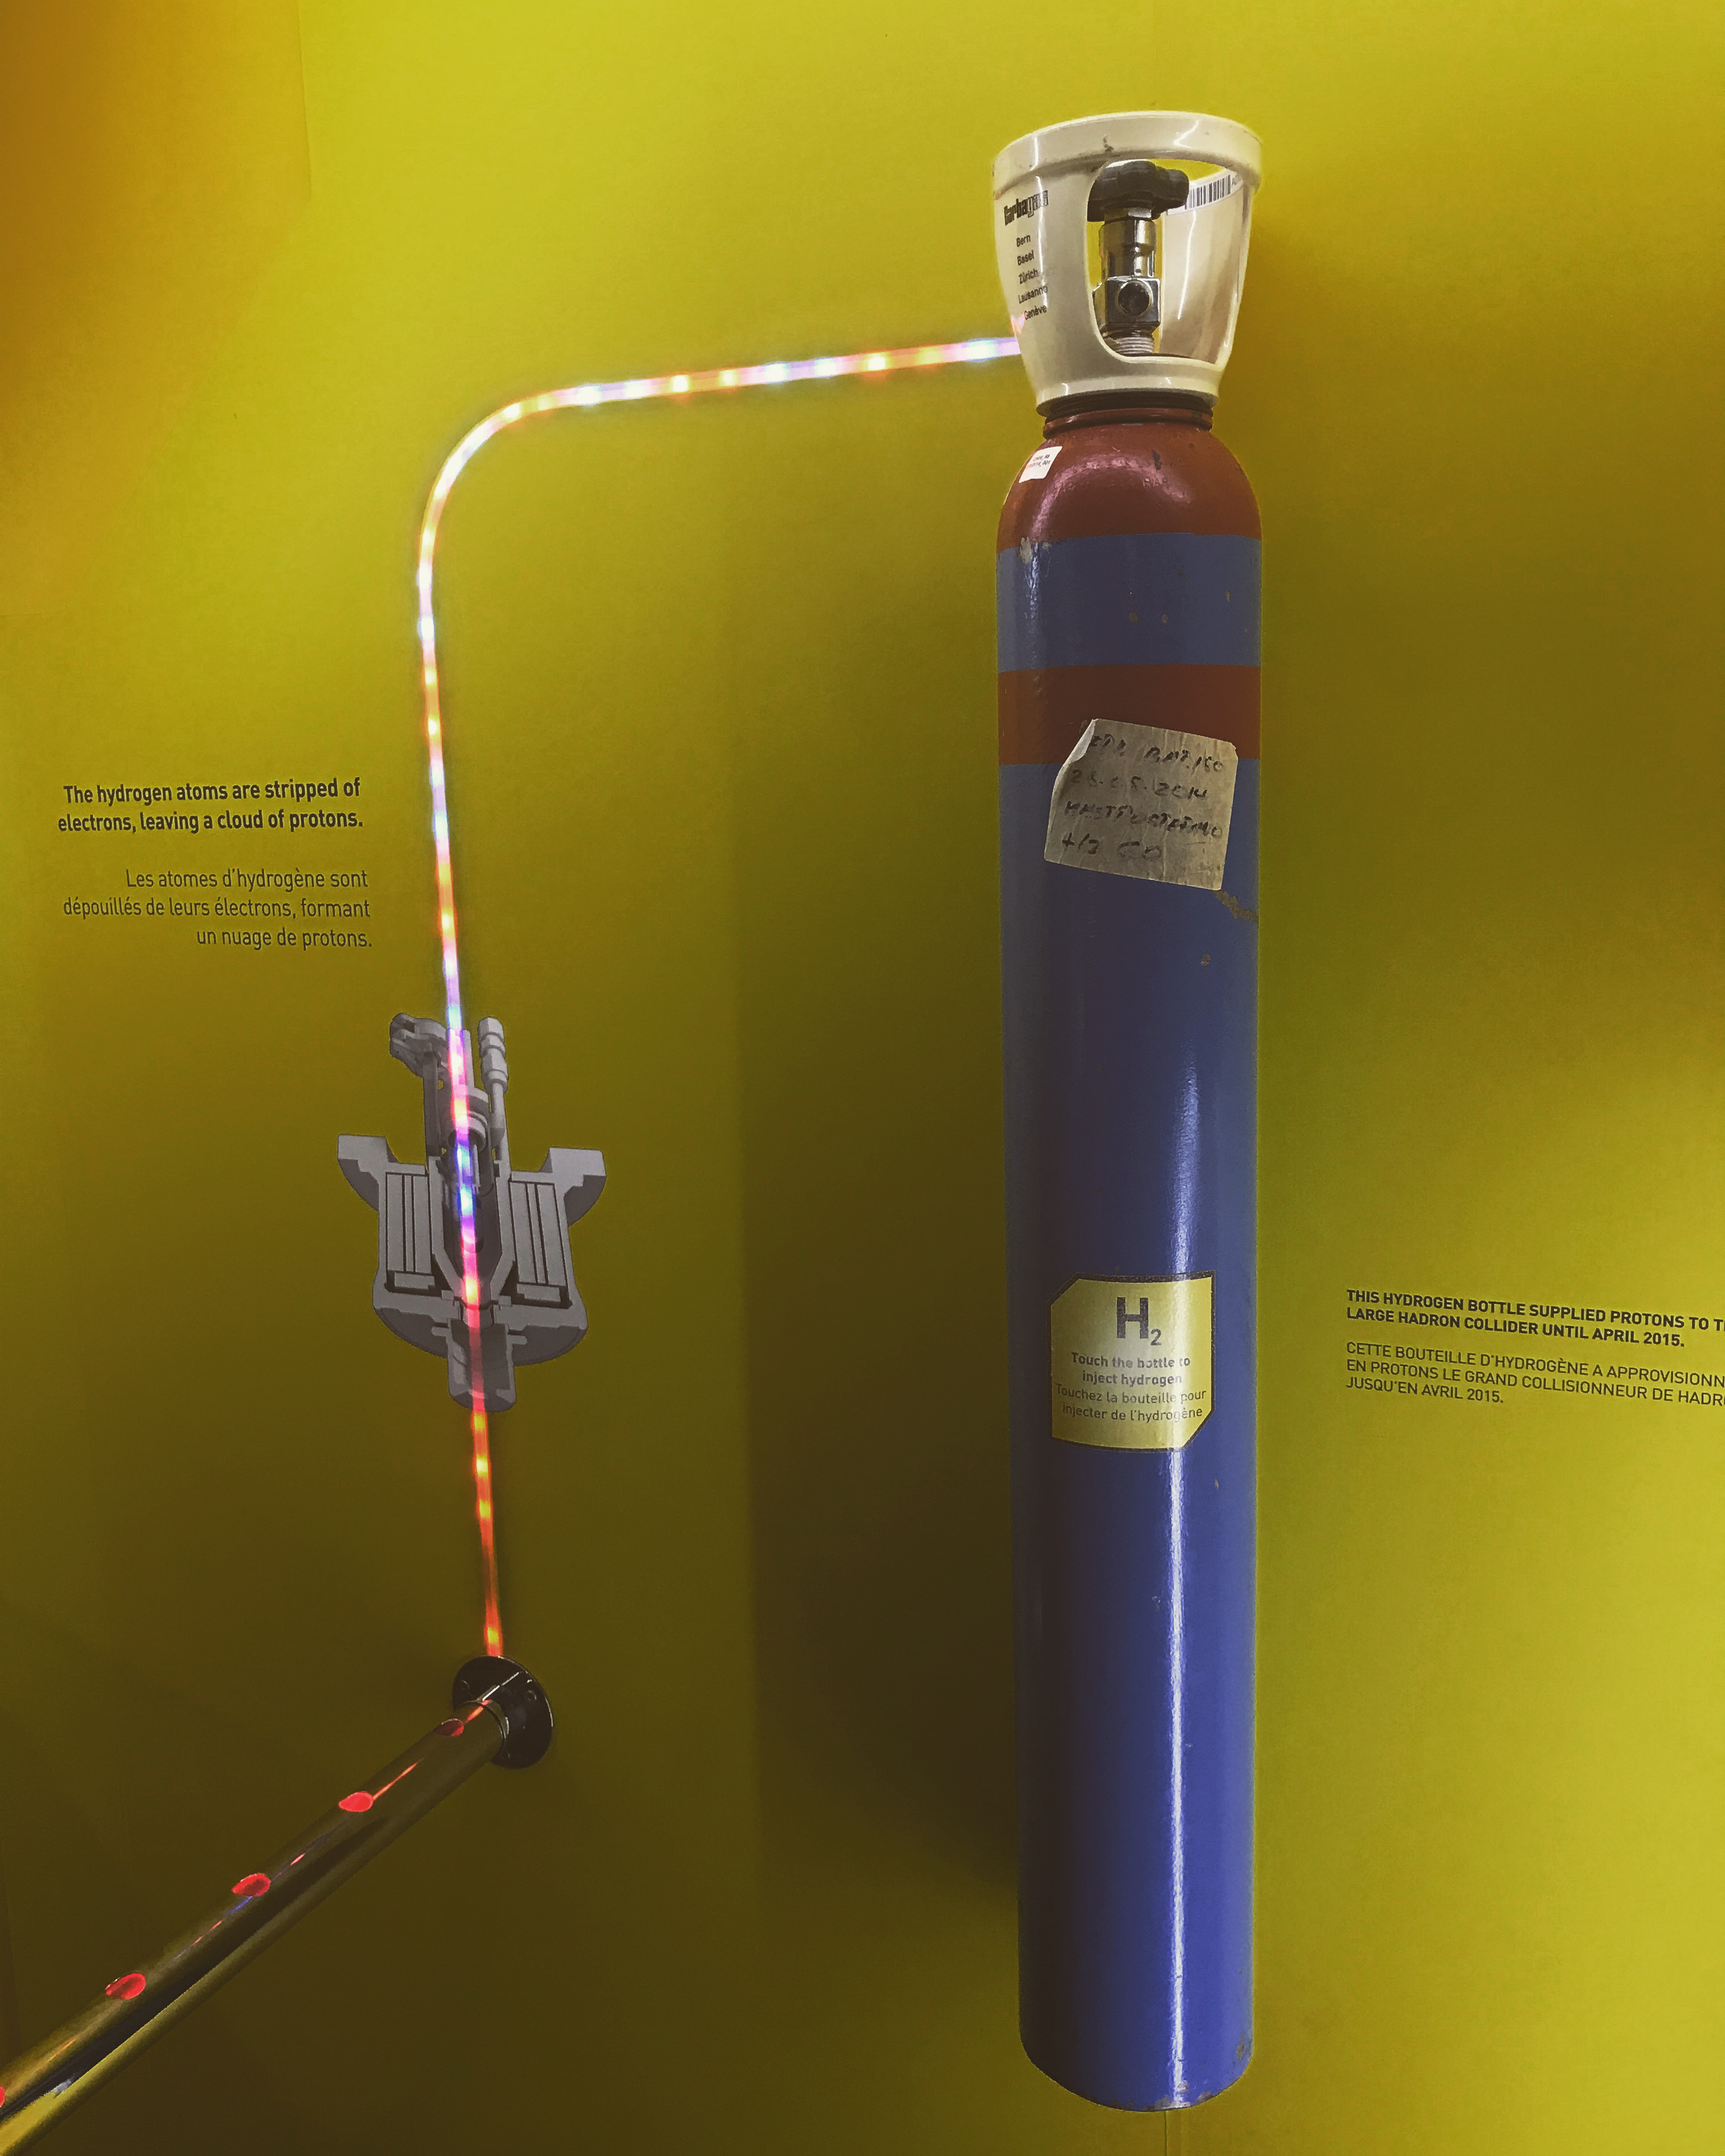
\includegraphics[scale=0.038]{fig/H2Bottle.JPG}
    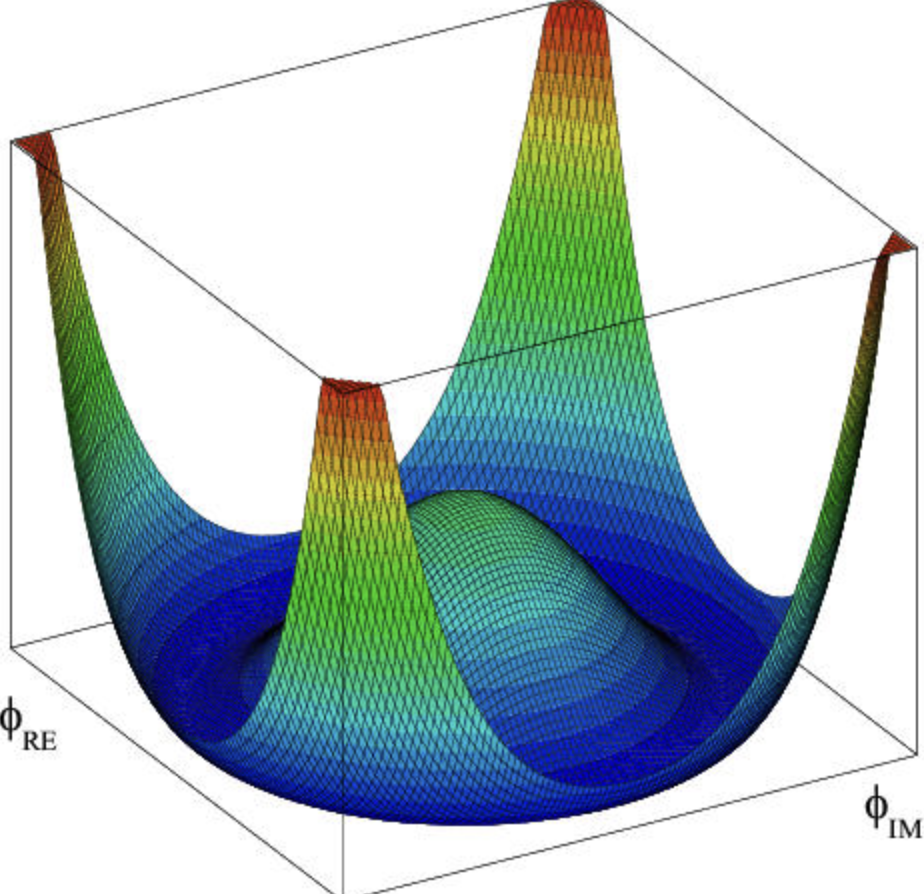
\includegraphics[scale=0.5]{fig/MexicanHat.png}
	\caption{The infamous "Mexican Hat" Higgs potential for the case of $\mu^2 <0$ and $\lambda >0$. There is a circle of minima of radius v.}
	\label{fig:MexicanHat}
\end{figure}

As mentioned earlier, the fermions gain mass via the Yukawa coupling of the single Higgs doublet $\phi$ with the fermions~\cite{Nguyen:HiggsMechanism}. In a nutshell, one can write a Yukawa coupling term in the lagrangian for a fermion:

\begin{equation}
    \label{eq:YukawaCouplingLag}
    \mathcal{L}_{\text{Yukawa}} = -g_f\bar{\psi_f} \phi \psi_f + h.c. 
\end{equation}

where g is a dimensionless coupling constant for some fermion $f$, $\psi_f$ is the fermion field and $\phi$ is the Higgs field. After spontaneous symmetry breaking, the Higgs field takes on the vacuum expectation value in Eq.~\ref{eq:VEV} the Lagrangian in Eq.~\ref{eq:YukawaCouplingLag}. For illustration, we do this for the first generation of fermions:

\begin{equation}
    \label{eq:YukVEV}
    \mathcal{L}_{\text{Yukawa}} =  \frac{f_e v}{\sqrt{2}} \left( \bar{e}_L e_R + \bar{e}_R e_L \right) + \frac{f_u v }{\sqrt{2}} \left( \bar{u}_L u_R + \bar{u}_R u_L \right) +  \frac{f_d v}{\sqrt{2}} \left( \bar{d}_L d_R + \bar{d}_R d_L \right), ...
\end{equation}
From here one can read off the masses as:
\begin{equation}
    \label{eq:FermionMasses}
   m_i = \frac{f_iv}{\sqrt{2}}, \quad i = e, u, d.
\end{equation}

One thing to note is that the neutrinos do not have right-handed partners in the SM and therefore could not acquire a mass term through Yukawa coupling \cite{Martin:1997ns}. 

On July 4, 2012, the CMS and ATLAS experiments independently announced the discovery of a particle consistent with the Higgs boson. This landmark achievement, while significant, did not ``complete" the Standard Model in the sense of resolving all fundamental questions in particle physics. Rather, it confirmed one of the final pieces of the SM puzzle, highlighting that numerous unresolved questions and challenges remain which requires further the exploration of new theoretical frameworks to expand our understanding of the universe.

\section{Limitations of the Standard Model}~\label{sec:SMLimitations}

In this section, we briefly give an overview of a number of open questions in the Standard Model and discuss in more detail how the BSM models we are exploring play a role in addressing these open problems. 

\subsection{Open Problems in Brief}~\label{sec:Open Problems}
\begin{itemize}
    \item  \textbf{Hierarchy Problem}: The Standard Model struggles to explain the vast disparity in the strengths of the fundamental forces, particularly why gravity is incredibly weaker than the other forces in our four-dimensional spacetime.
    \item \textbf{Parameter Fine-tuning}: The Standard Model involves several "unnatural" parameters, such as the low mass of the Higgs boson. Adjusting these parameters to match experimental observations appears contrived, lacking a deeper theoretical explanation.
    \item  \textbf{Quantum Theory of Gravity}: While the Standard Model successfully describes the other fundamental forces through quantum field theories, it falls short in providing a consistent quantum field theory for gravity, a long-standing challenge in theoretical physics.
    \item \textbf{Dark Matter and Dark Energy}: The Standard Model accounts for only a tiny fraction, approximately 4$\%$, of the total matter-energy content of the universe. It fails to address the presence of dark matter and the mysterious dark energy, both of which dominate the universe's composition.
    \item \textbf{Baryon Asymmetry}: There is an unexplained imbalance between matter and antimatter in the universe, known as the baryon asymmetry, which the Standard Model does not elucidate.
    \item \textbf{Strong CP Problem}: The mathematical formulation of Quantum Chromodynamics (QCD) within the Standard Model predicts a violation of CP-symmetry in strong interactions, which contradicts experimental observations. CP-symmetry dictates that the laws of physics should remain unchanged when particles are replaced with their antiparticles (charge reversal), followed by a left-right flip (parity reversal).
    \item \textbf{Neutrino Masses}: Neutrinos, initially assumed to be massless in the Standard Model, have been observed to have tiny but non-zero masses through experimental evidence. The SM does not naturally incorporate these neutrino masses and mixing angles, necessitating an extension of the theory to accommodate them.
    
\end{itemize}

\subsection{Hierarchy and Naturalness}~\label{sec:HierarchyandNaturalness}

It is well-established at this point that the Standard Model is a work-in-progress specially at higher energy regimes. Extensions to the standard model are guided by the principle of the desert hypothesis which has the fundamental premise that there is no new physics between the electroweak unification scale at $m_{EW}\approx1$~TeV and near the Planck mass or the reduced Planck Scale $M_P\approx 10^{18}$~GeV where quantum gravitational effects become significant. This large gap between the two scales refers to the well-known ``hierarchy problem". 

Theorists however think that this desert, 16 orders of magnitude wide, might conceivably host a plethora of successive layers of new effective field theories (EFTs). Among these are the ADD Large Extra Dimensions~\ref{sec:ADDmodel}, the Clockwork Model~\ref{sec:CWmodel} and the Unparticles~\ref{sec:UnparticlesModel}, which could serve diverse purposes, including the initiation of dynamical symmetry breakings or providing explanations for the intricate patterns observed in fermion masses and mixings \cite{Arkani-Hamed:1998jmv}. While the hierarchy problem might not be a direct issue with the Standard Model it reflects unsettling consequences related to the "naturalness" of the Higgs mass. 

The Higgs boson, being the only scalar particle in the Standard Model, possesses a distinct property: its quantum corrections are quadratically sensitive to high energy scales. This issue arises from the substantial quantum corrections originating from the virtual effects of every particle or phenomena directly or indirectly that couples to the Higgs field \cite{Martin:1997ns}. The general form for the Higgs boson mass calculation is written as:

\begin{equation}
    \label{eq:HiggsMass}
    m^2_H = m^2_{bare} + \Delta m^2_{H}, 
\end{equation}

\begin{figure}[!htbp]
	\centering  
    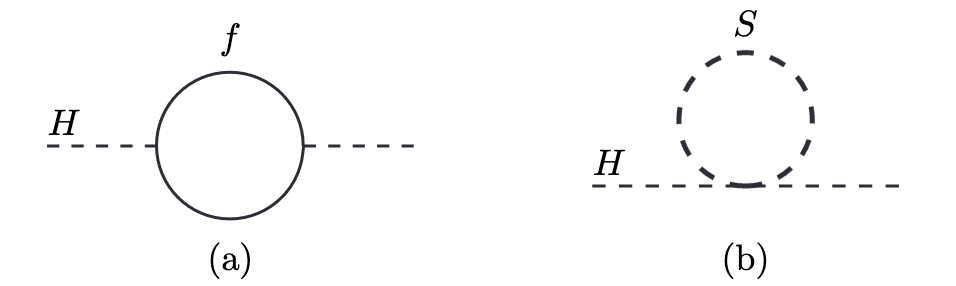
\includegraphics[scale=1.0]{fig/LoopCorrHiggs.png}
	\caption{One-loop quantum corrections to the Higgs squared mass parameter $m^2$, $H$ , due to (a) a Dirac fermion $f$ , and (b) a scalar $S$ \cite{Martin:1997ns}. }
	  \label{fig:HiggsQuantumCorr}
\end{figure}

where $m_H$ is the Higgs boson mass measured to be $125$~GeV, $m_{bare}$ is the Higgs boson bare mass, and $\Delta m^2_{H}$ are the said quantum corrections. To illustrate the problem, consider a correction from a loop described by the Feynman diagram in Fig.~\ref{fig:HiggsQuantumCorr} containing a Dirac fermion of mass $m_f$ coming from a term in the lagrangian $-\lambda_fH\bar{f}f$, 

\begin{equation}
    \label{eq:HiggsMass}
    \Delta m^2_{H} = - \frac{|\lambda_f|^2}{8\pi^2} \Lambda^2_{\textnormal{cutoff}} + ...
\end{equation}

Here, $\Lambda_{\textnormal{cutoff}} = \Lambda_{UV}$ refers to the ultraviolet momentum cutoff that is used to regulate the loop integral. It is also the energy scale at which new physics emerges. We can surmise that the SM is an EFT or a low-energy QFT approximation of some higher-energy theory which may include gravity and it is valid up to some cutoff scale. When bridging the hierarchy gap, $\Lambda_{\textnormal{cutoff}} \rightarrow \Lambda_{Planck}$, this contribution becomes too large, notwithstanding that these contributions add up for each fermion in the SM. At the $\Lambda_{Planck}$ scale, the bare mass and the quantum corrections would have to cancel over 30 orders of magnitude to match the measured value of the Higgs at 125 GeV. It seems that these quantum corrections have to be finely tuned and canceled out with an incredible degree of precision. This fine-tuning seems unnatural because it suggests that the observed Higgs mass is a delicate balance between the tree-level mass and the quantum corrections. In other words, it appears unlikely that nature would naturally set the Higgs mass to this specific value, given the sensitivity of the corrections to it. This is known as the Higgs naturalness problem.

\section{Beyond Standard Model Non-resonant Signals}~\label{sec:BSMNonReso}
The hierarchy and naturalness problem necessitated extensions to the Standard Model of which the primary and uncontested early candidate was Supersymmetry (SUSY). SUSY posits the existence of yet-to-be-discovered fermionic (bosonic) superpartners to the known bosons and fermions. With this framework, the strong, electromagnetic and weak coupling constants could be extrapolated and converge at a point just below the Planck Scale \cite{Martin:1997ns}.

In 1998, authors Nima Arkani-Hamed, Savas Dimopoulos, and Georgi Dvali (ADD), proposed a new framework\cite{Arkani-Hamed:1998jmv, Arkani-Hamed:1998sfv} that has a diametrically opposing premise from SUSY. They asserted that there is no desert between the electroweak scale and the Planck scale. Instead, they hypothesize the existence of additional $n_{ED}$ spatial dimensions with a radius $R$ which modifies the fundamental Planck Scale, which transforms the fine-tuning dilemma into a question of dynamics and geometry \cite{5LittleStringTheoryAtATeV}. With this approach, they also showed that the weakness of gravity could be explained by the existence of these extra dimensions in which only gravity propagates. Additionally, it has been shown~\cite{Dienes:1998vg, Dienes:1998vh} that these extra dimensions naturally lead to the unification of the coupling strengths at scales substantially below the usual GUT/ Planck scale. 

The idea of extra spatial dimensions is not entirely new. It has a historical precedent dating back to the 1920s, notably explored by Kaluza and Klein as an attempt to unify the fundamental forces~\cite{Kaluza:1921tu, Klein:1926fj, Klein:1926tv}. In the 1980s, string theory revisited this concept as a requirement for a consistent theory of quantum gravity, with the dimensions compactified near the Planck scale and therefore not testable experimentally ~\cite{ParticleDataGroup:2020ssz}. While the initial endeavour faltered, the Kaluza-Klein (KK) formalism remains valuable today, albeit with modified forms and assumptions. 

A year after the ADD model was proposed, Randall and Sundrum introduced a groundbreaking approach wherein the extra dimension has a warped geometry in a five-dimensional negatively curved, Anti-de Sitter (AdS) spacetime, with a compactification scale near 1/TeV. This model explained the electroweak scale's smallness relative to the Planck scale by invoking a gravitational redshift factor that is intrinsic to the warped AdS metric. Initially conceived for gravity alone, it was soon evident that the Standard Model's gauge fields and fermions could also propagate within these five-dimensional spacetime regions~\cite{Randall:1999ee, Randall:1999vf, ParticleDataGroup:2020ssz}. 

Around a decade later, additional frameworks that try to solve the hierarchy problem through various geometries and or field dynamics were proposed. One model is the Continuum Clockwork Model~\cite{2Clockwork} which has a remarkable resemblance to the Linear Dilaton theory of Little String Theory~\cite{5LittleStringTheoryAtATeV}. At some limit, we show that it is equivalent to the ADD LED and the RS model. Another is the Unparticles Scenario which explores the possible existence of unconventional scale-invariant fields and interactions in particles. While the Unparticles~\cite{Georgi_2007unpar, Georgi:2007o, Georgi:2007si} framework is distinctly different from the other aforementioned models, they mimic the phenomenology of extra dimensions which look like an almost continuum of broad or closely-spaced resonances ~\cite{Folgado:2020utn}. In the succeeding parts of this chapter, we explain explain some salient mathematical and phenomenological features of the ADD Large Extra Dimensions~\ref{sec:ADDmodel}, the Clockwork/Linear Dilaton~\ref{sec:CWmodel} and the Unparticles~\ref{sec:UnparticlesModel} - the non-resonant models we explore in this analysis.

\subsection{ADD Large Extra Dimensions}~\label{sec:ADDmodel}
In the ADD scenario, the hierarchy problem is resolved via the existence of $n$ extra dimensions with a finite radius R. This is illustrated in Fig.~\ref{fig:LEDSketch}. The apparent weakness of gravity is also explained because it propagates in the bulk or the extradimensional volume. In effect, the enormity of the Planck scale becomes simply a consequence of the large size of the extra dimensions.

\begin{figure}
    \centering
    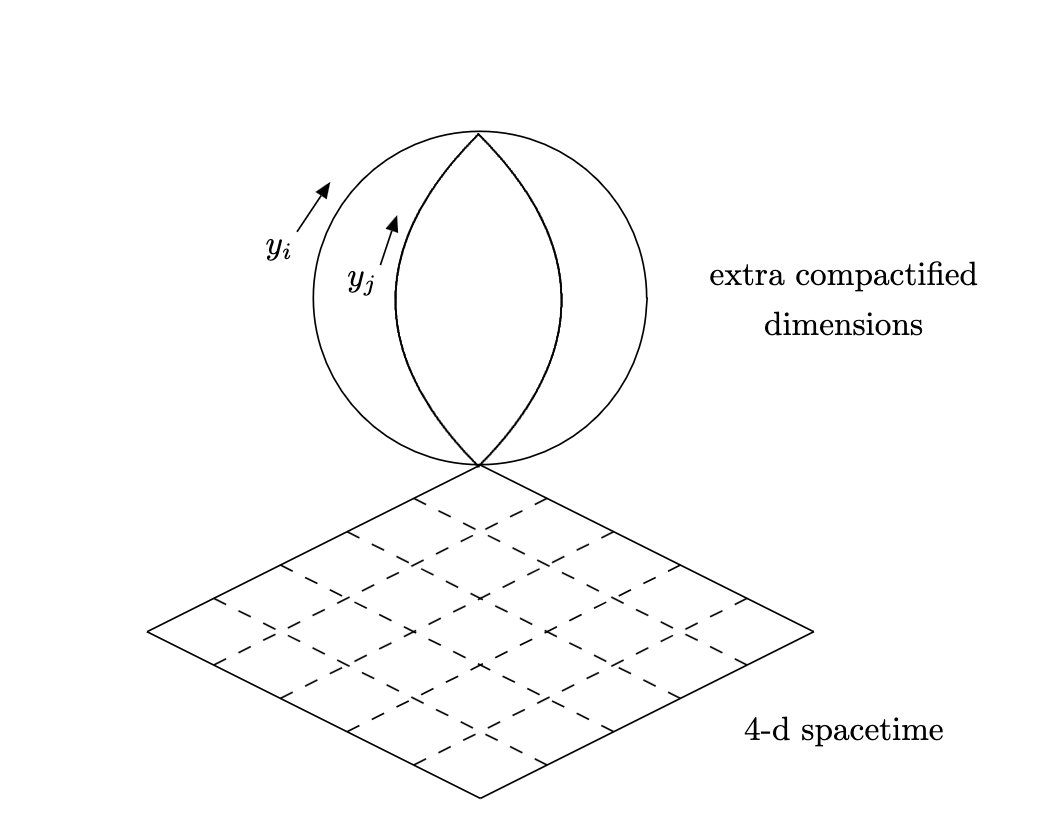
\includegraphics[scale=0.7]{fig/LEDsketch.png}
    \caption{LED Scenario Schematic where compactified extra dimension goes beyond our 4-dimensional spacetime where SM particles live.~\cite{Kribs:2006mq}}
    \label{fig:LEDSketch}
\end{figure}

With this as a guiding principle, a new fundamental scale, much closer than the Planck scale and therefore experimentally accessible, is established. 
The Planck scale in terms of this new scale $M_D$ can be written as:

\begin{equation}
    \label{eq:NewPlanckMass}
    M^2_{Pl} = M_{D}^{2+n}R^n.
\end{equation}

To illustrate this, we follow the ideas given in the first paper on the ADD LED scenario~\cite{Arkani-Hamed:1998jmv}. Here, all SM particles and gauge interactions are confined our 4-dimensional brane which is embedded in a larger 4+$N$-dimensional bulk space, with $N$ extra dimensions that are compactified in a sphere or torus of radius R, with volume $V_n =(2 \pi R)^n$. In this 4+$N$ world, the gravitational potential between two masses $m_1$ and $m_2$, a distance $r \ll R$ from one another will feel a gravitational potential dictated by Gauss's law:

\begin{equation}
\label{eq:GaussLaw4D+nShort}
    V(r) \approx \frac{m_1m_2}{M^{N+2}_{Pl(4+N)}}\frac{1}{r^{n+1}}}, (r \ll R).
\end{equation}

If these two masses are separated with a distance $r \gg R$ from one another, their gravitational flux is too weak to penetrate the the extra dimensions so the usual $1/r$ potential is obtained,

\begin{equation}
\label{eq:GaussLaw4D+nLong}
    V(r) \approx \frac{m_1m_2}{M^{N+2}_{Pl(4+N)}R^N}\frac{1}{r}, (r\gg R).
\end{equation}

Comparing the two equations, we get the effective 4-D $M_{Pl}$, 

\begin{equation}
\label{eq:Mplanck_MEW}
   M^2_{Pl} \approx  M^{2+N}_{Pl(4+N)}R^N.
\end{equation}

This is equivalent to Eq.~\ref{eq:NewPlanckMass}.

For the hierarchy problem to be solved, we set $M_{D}\approx M_{EW}\approx1$~TeV, and demand that $R$ the observed $M_{Pl}$ yields,

\begin{equation}
    R \sim 10^{\frac{30}{n} -17} \text{cm}}\times\left(\frac{1~TeV}{m_{EW}}\right)^{1+\frac{2}{n}}.
\end{equation}

When $n=1$, the radius R is approximately $10^{13}$ centimeters which leads to observable deviations to Newtonian gravity within the solar system. This is clearly ruled out. For all cases $n \geq 2$, R goes at sub-mm distances. These are cases currently being explored in collider experiments and astrophysical and cosmological constraints are being set on the reduced Planck scale $M_D$ ~\cite{ParticleDataGroup:2020ssz}.

It's important to acknowledge that while the existence of large extra dimensions can address the hierarchy problem, it introduces another challenge in the form of a finely-tuned parameter: the size of the extra dimensions, R. As discussed earlier, R must be carefully chosen to match the 4D Planck scale and ensure that $M_D$ is on the Electroweak (EW) scale. This requirement replaces the need for fine-tuning of the bare Higgs boson mass. Regardless of our confidence in the ADD model specifically, it inspires a range of experiments to detect potential deviations from the Standard Model (SM). 

\subsubsection{ADD Phenomenology}

The Einstein-Hilbert Action for the ADD model can be 
pieces~\cite{Kribs:2006mq}: 

% The action of the ADD model can be decomposed into two pieces~\cite{Kribs:2006mq}: 

\begin{equation}
    \label{eq:ADDAction}
    S = S_{bulk} + S_{brane}
\end{equation}

where we are assuming that there is only one brane where the SM fields exist. The bulk action is just the Einstein-Hilbert Action for $4+n$ dimensional gravity:

\begin{equation}
    \label{eq:SBulkADD}
     S_{bulk} = -\int d^{(4+n)}x \sqrt{g^{4+n}}M^{n+2}_{D} \, R^{(4+n)}, 
\end{equation}

where $R^{(4+n)}$ is the higher-dimensional Ricci curvature scalar. 

In terms of the lagrangian density for the lagrangian density of the bulk fields $\phi(x,\Vec{y})$, we have:
\begin{equation}
    \label{eq:SBulkADD}
     S_{bulk} = \int d^{4}xd^ny \sqrt{|g^{4+n}|} \mathcal{L}(\phi(x,\Vec{y})), 
\end{equation}, 

Here $x$ stands for the (3+1) coordinates of the brane and $y$ is for the n extra dimensions ~\cite{Perez-Lorenzana:2005fzz}. On the other hand the action for the Brane Fields, $\xi(x)$ is written as
\begin{equation}
    \label{eq:SBraneADD}
     S_{Brane} = \int d^{4}xd^ny \sqrt{|g^{4+n}|} \mathcal{L}(\xi(x)) \delta^{n}(\Vec{y}-y_0), 
\end{equation}
where the use of the delta density promotes the fields to a higher dimensional expression. The brane is taken to be at a position $\Vec{y}=\Vec{y_0}$.

The line element in the bulk is 

\begin{equation}
    \label{eq:ADDBulkMetric}
    ds^2 = g^{4+n}_{\mu\nu}dx^{\mu}dx^{\nu}.
\end{equation}

The ADD model assumes spacetime is flat, in contrast to the RS model where it is warped. Hence, the metric tensor $g_{\mu\nu}$, the quantity that encodes the curvature of spacetime, can be expanded about flat spacetime with 4D metric fluctuations $h_{\mu\nu}$,

\begin{equation}
    \label{eq:ADDBulkMetric}
    ds^2 = (\eta_{\mu\nu} + h_{\mu\nu})dx^{\mu}dx^{\nu}-r^2d\Omega^2(n), 
\end{equation}

where $d\Omega_{(n)}$ are n-dimensional toroidal coordinates. Following the steps in ref.~\cite{Kribs:2006mq}, we can integrate out the higher dimensions and arrive at the result

\begin{equation}
    \label{eq:MplanckVolume}
    M^2_{\pl} = M^{n+2}_D (2 \pi r)^n,
\end{equation}

which is the same result in Eq.~\ref{eq:Mplanck_MEW} we quote in the previous section. The arbitrary metric fluctuations about the flat space time, $h_{\mu\nu}$ could be interpreted as the higher dimensional graviton which are laid out in more detail Refs.~\cite{Perez-Lorenzana:2005fzz,Kribs:2006mq, Giudice:1998ck}. Defining higher dimensional coordinates $y_i$, and imposing a periodic boundary conditions, $y_i \rightarrow y_i + 2\piR$ due to the compactifications of the extra dimensions, we have the expansion of the higher dimensional graviton in terms of the 4D Kaluza-Klein (KK) fields:

\begin{equation}
    \label{eq:KKexpansion}
    h_{\mu\nu} = \sum_{m1 = -\infty}^{\infty} ... \sum_{mn = -\infty}^{\infty} \frac{h^{(m)}_{\mu\nu}(x)}{\sqrt{V_n}} e^{i\frac{m_jy_j}{R}},
\end{equation} 

where $h^{m}$ is shorthand for $h^{(m_1,m_2,...m_n)}$. 
These KK graviton excitations or "tower" results from the coupling of the graviton to SM fields. Each of these KK modes couple to the stress-energy tensor of the SM field by the strength of gravity. The KK mass is given by $m^2_n = m^2 + \frac{k^2}{r^2}$. This mass spectrum, illustrated in Fig.~\ref{fig:KKmassSpectrum}, can be much less than the detector resolution. In this CMS analysis, we look at the invariant diphoton mass spectrum illustrated by a result from a previous analysis in Fig.~\ref{fig:CMSModelDiphotonInvMass}~\cite{CMS:2011uvc}. The closely spaced KK modes are therefore predicted to appear as a continuum excess in the diphoton mass spectrum. 

\begin{figure}
    \centering
    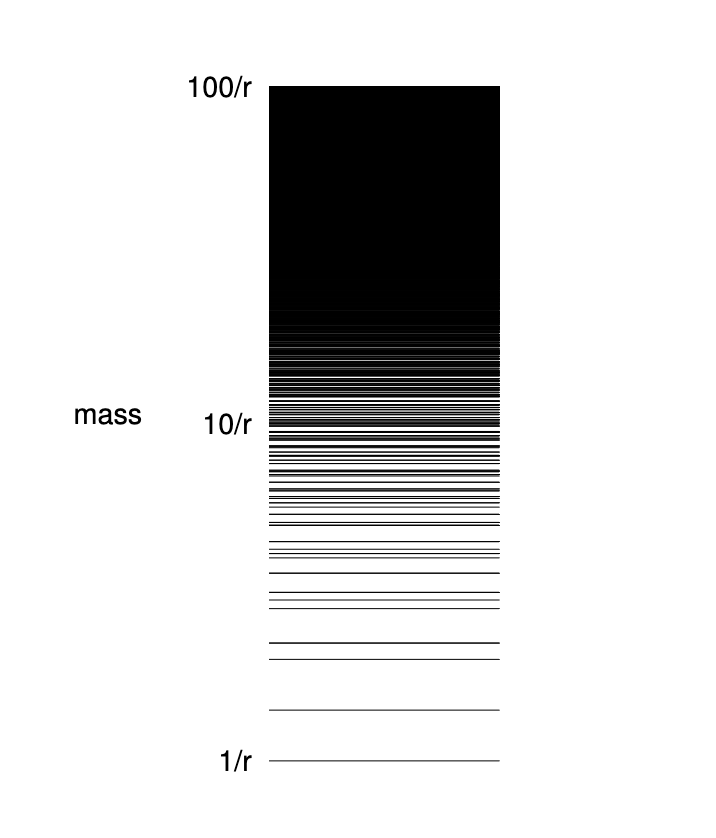
\includegraphics[scale=0.4]{fig/KKMassSpectrum.png}
    \caption{Mass spectrum for KK gravitons for $n=2$. These discrete KK states are closely spaced together and gets closer together and appear as a continuum.}
    \label{fig:KKmassSpectrum}
\end{figure}


\begin{figure}
    \centering
    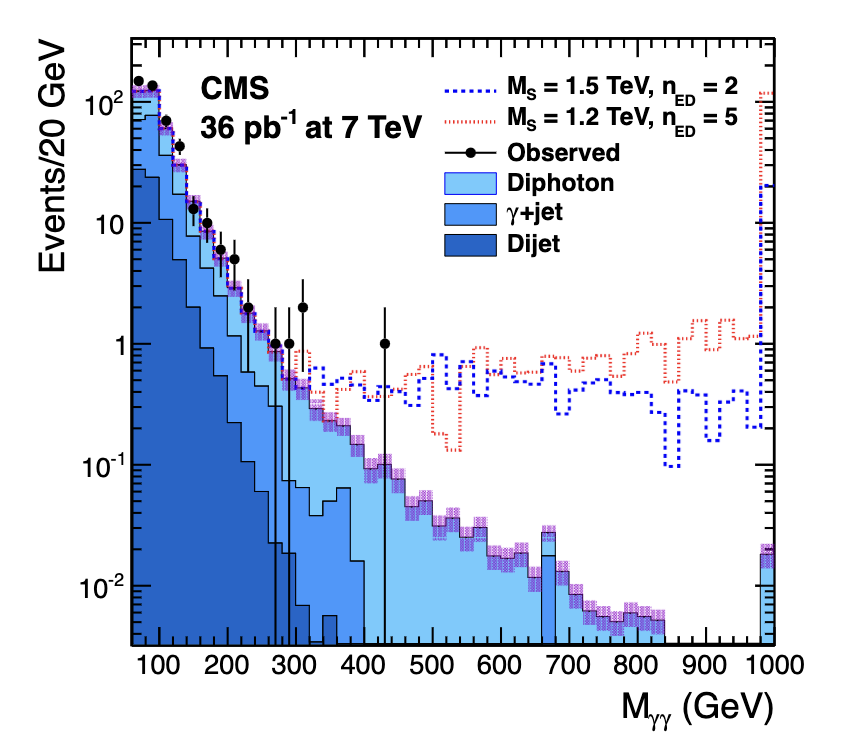
\includegraphics[scale=0.6]{fig/InvariantMass.png}
    \caption{A CMS result~\cite{CMS:2011uvc} using data from $\sqrt{s} = 7$~\TeV pp-collisions which shows a comparison of the invariant mass spectrum predicted for the Standard Model diphoton production in light blue, overlayed with a continuous spectra for two Large Extra Dimensions signal points shown in dashed lines. The observed data and additional background predictions from $\gamma+$jet and dijet events are also shown in various markers indicated in the legend.}
    \label{fig:CMSModelDiphotonInvMass}
\end{figure}


Since there are an infinite number of KK modes, an ultraviolet (UV) cutoff $M_s$ is introduced to get a non-diverging cross-section. The cross-sections for the virtual graviton exchange (see Fig.~\ref{fig:FeynmanDiagramUG}) for various parameters are shown in in Appendix~\ref{ch:appendix_signal_monte_carlo}. Any contributions above the cutoff scale $M_s$ is set to zero. The total cross-section is a combination of the contributions from the SM, ADD as well as the interference between the SM and ADD:

\begin{equation}
\sigma_{total} = \sigma_{SM} + \frac{\mathcal{F}}{M^4_{S}} \sigma_{int}+\frac{\mathcal{F}}{M^8_{S}} \sigma_{ADD} 
\label{eq:totalADDxsec}
\end{equation}

Here, $\mathcal{F}$ is parameter which allows us to translate our results in the different conventions for the ADD model that are found in literature. Here we  consider the GRW~\cite{Giudice:1998ck}, HLZ~\cite{Han:1998sg} and the Hewett~\cite{Hewett:1998sn} conventions where we have, 

\begin{equation}
\mathcal{F}=
    \begin{cases}
        1 & \text{if } \textnormal{GRW} \\
        log\left(\frac{M^2_s}{\hat{s}}\right) & \text{if } n_{ED} = 2 \\
        \frac{2}{n_{ED} - 2} & \text{if } n_{ED} > 2 \\
        \pm \frac{2}{\pi} & \text{if } \textnormal{Hewett}.
    \end{cases}
    \label{eq:KKConventions}
\end{equation} 

Here $\hat{s}$ is the centre-of-mass energy of the colliding partons. It is important to note that the GRW and the HLZ conventions interfere constructively while the Hewett could either interfere constructively (+) or destructively (-), according to the signs in Eq.~\ref{eq:KKConventions}. Later in Ch.~\ref{ch:SignalModelling}, $M_s$, is replaced by $\Lambda_{T}$ whose equivalence varies by convention.

% \begin{equation}
% \mathcal{F}=
%     \begin{cases}
%         1 & \text{if } x \in \mathbb{Q}\\
%         log\left(\frac{M^2_s}{\hat{s}}\right) & \text{if } x \in \mathbb{R}\setminus\mathbb{Q}
%     \end{cases}
% \end{equation}



\begin{figure}
    \centering
    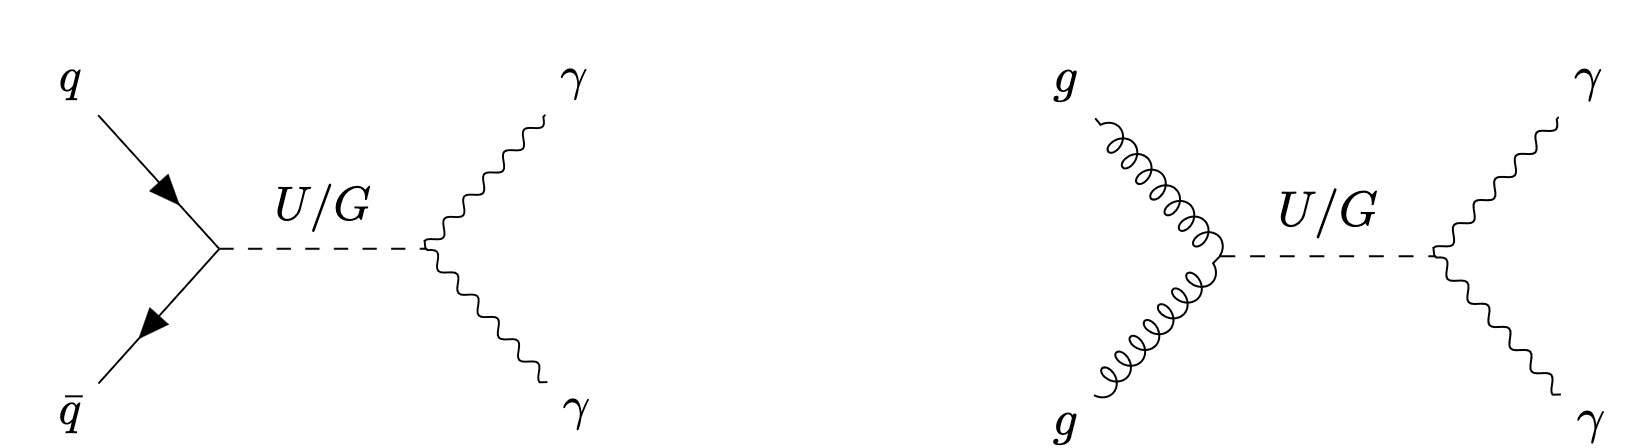
\includegraphics[scale=0.5]{fig/FeynmanDiagramUG.png}
    \caption{Feynman Diagrams for virtual graviton or Unparticle exchange in the diphoton channel $\gamma\gamma$ through quark annihilation (left) and gluon fusion (right).}
    \label{fig:FeynmanDiagramUG}
\end{figure}

\subsection{Clockwork/ Linear Dilaton}~\label{sec:CWmodel} 
A more recent model that has been proposed is the Continuum Clockwork model which is equivalent to the Linear Dilaton theory in 5D. The CW/LD model is distinct but related to the more known extra-dimensional models which are the ADD LED and the RS Graviton scenarios. In the clockwork picture, the hierarchy is solved by introducing a continuum of clockwork fields which interact with each other. Inspired by gears transmitting energy, they are arranged in a way that the fields/particles associated have increasing masses/energy scales as you move along the chain as seen in Fig.~\ref{fig:ClockworkSchematic}.
This general mechanism can take large effective interaction scales from dynamics occuring at much lower energies. These ``gears" could also be interpreted as N copies of some particle content laid out on a one-dimensional lattice in theory space. In the continuum limit this lattice interpreted as a physical extra dimension and the gears are the KK modes~\cite{2Clockwork}. 

The basic mathematical setup of the CW/LD follows from Ref.~\cite{Giudice:2017fmj}. A 5D space is considered in which the extra dimension is a circle parametrized by $y$ where $- \pi R \leq y \leq \pi R$. The SM or TeV brane is set at $y = 0 $, whereas the Planck brane is set at $y = y_p = \pi R$. With a $Z_2$ orbifold symmetry, $y\leftrightarrow-y$ are identical. The full action in the Einstein frame is a sum of the SM action, the Bulk action and additional terms account for the extrinsic curvature of the two boundaries and the scalar potentials at the TeV and Planck branes near their local minima.

\begin{figure}
    \centering
    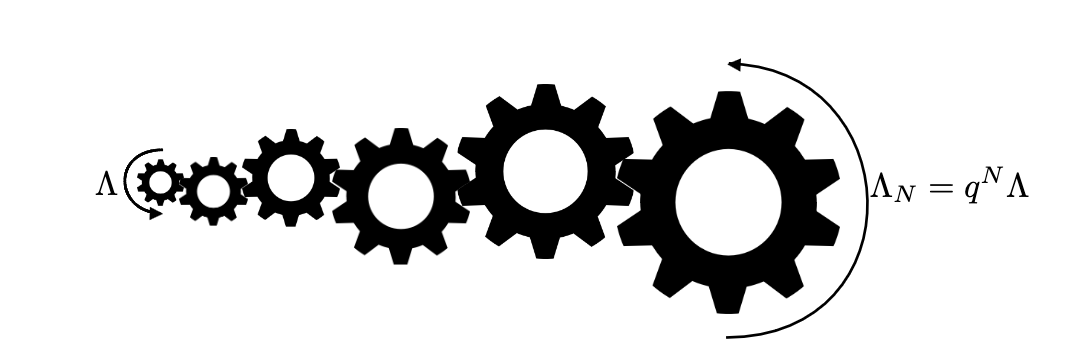
\includegraphics[scale=0.5]{fig/ClockworkSchematic.png}
    \caption{A schematic representation of the clockwork mechanism increasing the interac-
tion scale of a non-renormalisable operator~\cite{2Clockwork}. }
    \label{fig:ClockworkSchematic}
\end{figure}

In this scenario, Einstein's equations and the dilaton equation of motion are solved by the metric,

\begin{equation}
    \label{eq:CWMetric}
    ds^2 = e^{\frac{4}{3}ky}g_{\mu\nu}dx^{\mu}dx^{\nu} + dy^2.
\end{equation}

Taking into account the metric in Eq.3.34 of Ref.~\cite{2Clockwork} which describes the graviton fluctuations around the 4D Minkowski space, we can write the decomposed graviton states as:

\begin{equation}
    \label{eq:GravitonEigenstates}
    h_{\mu\nu}=  \sum_{n = 0}^{\infty} \frac{\tilde{h}_{\mu\nu}(x) \Psi_n(y)}{\sqrt{\pi R}}.
\end{equation}

If we suppose that the SM fields localized at $y=0$, we can write the interaction lagrangian as 


\begin{equation}
    \label{eq:GravIntclockwork}
    \mathcal{L} = -\frac{h_{\mu\nu}(x,0)T^{SM}_{\mu\nu}(x)}{M^{3/2}_5} = -\sum_{n = 0}^{\infty} \frac{\tilde{h}_{\mu\nu}(x) T^{SM}_{\mu\nu}(x)}{\Lambda_n}, 
\end{equation}

where $T^{\textnormal{SM}}_{\mu\nu}(x)$, is the SM energy-momentum tensor and $\Lambda_n$ is the effective scale of interaction. In more detail these are written as, 

\begin{equation}
\label{eq:TuvAndIntScale}
T^{SM}_{\mu\nu}(x) &= -2\frac{\partial \mathcal{L}^{SM}}{\partial g_{\mu\nu}} + g_{\mu\nu}\mathcal{L}^{\textnormal{SM}} ; \quad
\Lambda_n &\equiv \frac{\sqrt{\pi R M^{3/2}_5}}{\psi_n(0)}.
\end{equation}

With this metric and the action, (see Appendix A of Ref.~\cite{2Clockwork}) one can derive the analogue to Eq.~\ref{eq:NewPlanckMass},

\begin{equation}
    \label{eq:MP_CW}
    M^2_{P} \approx \frac{M^3_5}{k} \left(e^{2 \pi kR-1}\right),
\end{equation}

where $M_5$ is the fundamental scale or the 5D reduced Planck Mass $M_D$.
This is the scale at which the theory must be UV-completed and it is assumed to be close to $M_{EW}$. Here, $M_P$ is an illusion caused by exponential factor, similar to the RS scenario. Using the Eq.~\ref{eq:TuvAndIntScale}, Eq.~\ref{eq:MP_CW}, as well as Eq.3.16 and 3.17 of Ref.~\cite{2Clockwork}, the effective scales of gravitational interaction are:
\begin{equation}
\label{eq:CWKInteractionScales}
\Lambda_0 &= M_P; \quad
\Lambda_n &= \sqrt{M^3_5 \pi R \left(1 + \frac{k^2 R^2}{n^2}  \right)}.
\end{equation}

To account for hierarchy, one needs to choose an appropriate $kR$ and expand the natural logarithm

\begin{equation}
    \label{eq:kRCW}
    kR \approx \frac{1}{\pi} ln\left(\frac{M_P}{M_5} \sqrt{\frac{k}{M_5}}\right) \approx 10 + \frac{1}{2\pi}ln\left(\frac{k}{\textnormal{TeV}}\right)-\frac{3}{2\pi}ln\left(\frac{M_5}{10\textnormal{TeV}}\right).
\end{equation}

Here, $k$ is a mass parameter called the ``clockwork spring" which measures the effectiveness of the clockwork mechanism. A flat metric corresponds to $k = 0$. As described in the original paper, the extra dimension is discretized by choosing $y_j = ja$, where $j = 0,...,N$. The lattice spacing $a$ is such that $Na = \pi R$. While this construction resembles fields in a deconstructed flat extra dimension, there is a critical difference which comes from how each link breaks the symmetry of a single gear site. A parameter q treats the site $j+1$ and the site $j$ (with $j = 0,..., N - 1$) asymmetrically. It's important to note that we can establish a total of $N$ connections among the $N + 1$ available sites. As a consequence, one site retains its masslessness. For q to remain $y$-independent and for $q^N$ to give a finite but non-trivial clockwork behavior, as the number of sites approaches infinity, we set 

\begin{equation}
    \label{eq:qEq}
    q^N = e^{k \pi R}.
\end{equation}

The excitations have a similar form with the large extra dimensions, where at the large N limit, we have

\begin{equation}
\label{eq:CWKKModes}
m^2_0 &= 0; \quad
m^2_n &= k^2 + \frac{n^2}{R^2} + \frac{O(1)}{N}, \quad n = 1, \ldots, N
\end{equation}

which appears as a continuous spectrum like the ADD LED but with evenly distributed energy levels and mass-squared splitting equal to the inverse radius-squared. However, we will see later in Ch.~\ref{ch:SignalModelling} that the spectrum shifts by an amount equal to the clockwork spring constant k, introducing a mass gap~\cite{2Clockwork}. 

\subsection{Unparticles Model}~\label{sec:UnparticlesModel}
The two previous models propose scenarios which address the hierarchy problem via the existence of extra spatial dimensions. The Unparticles~\cite{Georgi_2007unpar} model on the other hand, addresses the hierarchy problem by introducing a new energy scale related to a yet-to-be-seen scale-invariant Banks-Zaks ($\mathcal{BZ}$) sector where ``unparticle stuff" live. If this sector exists, there are measureable effects coming from the interactions between the Standard model particles and the these hidden sector Unparticles. This has particular consequences with the Higgs naturalness problem - a dilemma where the Higgs mass receives quantum corrections that are quadratically sensitive to the energy scale of new Physics. Instead of the scale being at $M_P$, this new scale could be much closer via the existence of the $\mathcal{BZ}$ and the unparticle-SM interactions could help redistribute the quantum corrections and potentially reduce the fine-tuning problem~\cite{Kikuchi:2007qd}.

While not directly related to this dissertation, the Unparticles model can also potentially address issues related to flavor physics and CP violation via new interactions through the hidden sector and modifications in the flavor-changing and CP-violating processes that could still be consistent with experimental observations~\cite{Georgi_2007unpar, Chen:2007vv,Freitas:2007ip, Zwicky:2007vv}.

In the first paper by Georgi~\cite{Georgi_2007unpar}, the scale-invariant $\mathcal{BZ}$ sector must interact weakly with the Standard Model. Such a sector could not have particles of definite non-zero mass as mass terms explicitly breaks scale invariance.
It only holds ``Unparticles" which is a hazy concept that is different from our familiar notion of particulate notion of particulate matter. However, using a low-energy ``Effective field theory" (EFT), some phenomenological exploration is possible. 

% Thus the domain of utility of an effective theory is necessarily bounded
% from above in energy scale

In general, direct searches are only possible if the form of the BSM theory is established, but an EFT~\cite{Georgi:1993mps} approach allows us to quantify deviations from SM predictions of known particles without introducing additional assumptions about the BSM theory. The only assumption made is that the BSM theory will faithfully reproduce the SM in the regime where it is already empirically validated. As mentioned earlier, we can surmise that the SM is an effective field theory of some higher-energy theory which is valid to some cut-off energy scale $\Lambda$. 

For the Unparticles scheme, the new higher energy theory contains the SM fields and the $\mathcal{BZ}$ fields, which has a nontrivial IR fixed point. The two sets of fields interact via the exchange of particles with a large Mass Scale $M_{\mathcal{U}}$. Below this scale the interaction can be described by non-renormalizable couplings suppressed by powers of  $M_{\mathcal{U}}$ and we can write the interacting lagrangian in the following form

\begin{equation}
    \label{eq:LagIntUnpar}
    \mathcal{L}_{int} = \frac{1}{M^k_{\mathcal{U}}} \mathcal{O}_{SM}\mathcal{O}_{\mathcal{BZ}}
\end{equation}

where $\mathcal{O}_{SM}$  is an operator with mass dimension $d_{SM}$ that is built out of SM fields and $\mathcal{O}_{\mathcal{BZ}}$ is an operator $d_{\mathcal{BZ}}$ built out of $\mathcal{BZ}$ fields. The exponent $k= d_{SM} + d_{BZ}-4$.

At energy $\Lambda_{\mathcal{U}}$, the $\mathcal{BZ}$ sector emerges and it is expected to be conformal. However, this coupling transmutes as the energy increases to $\Lambda_{\mathcal{U}}$ as the scale invariance or conformal invariance is expected. In the effective theory below  $\Lambda_{\mathcal{U}}$, the $\mathcal{O}_{\mathcal{BZ}}$ operators match unto Unparticle operators and the interactions match onto the following form

\begin{equation}
    \label{eq:LagIntUnparMatch}
    \mathcal{L}_{int} =  \frac{C_{\mathcal{U}}\Lambda^{d_{BZ}-d_{SM}}_{\mathcal{U}}}{M^k_{\mathcal{U}}}\mathcal{O}_{SM}\mathcal{O}_{\mathcal{U}} = 
    \frac{\lambda}{ 
    \Lambda_{\mathcal{U}}^{ d_{\mathcal{U}}+d_{SM}-4}}} }\mathcal{O}_{\mathcal{U}}\mathcal{O}_{SM}
\end{equation}

Here $\mathcal{O}_{\mathcal{U}}$ is the Unparticle operator with dimension $d_{\mathcal{U}}$, $\lambda$ is the coupling constant between SM and $\mathcal{BZ}$. Georgi observed that the Unparticle mass spectrum looked like a $d_{\mathcal{U}}$ number of invisible massless particles. Following the arguments from Ref.~\cite{Georgi_2007unpar, Cheung:2007ap, CheungEtAl:2007}, scale invariance can be used to fix the two-point functions of these unparticle operators to show this effect. Consider a the vacuum matrix element, $\mathcal{O}_{\mathcal{U}}$,

\begin{equation}
\begin{align*}
    \langle 0|\mathcal{O}_{U}(x)\mathcal{O}_{U}^\dagger (0)|0\rangle 
    &= \langle 0|e^{i\hat{P}\cdot x}O_U(0)e^{-i\hat{P}\cdot x}O_U^\dagger (0)|0\rangle \\
    &= \int d\lambda \int d\lambda' \langle0| \mathcal{O}_{U}(0)|\lambda'\rangle 
    \times \langle \lambda'| e^{i\hat{P}\cdot x} |\lambda\rangle 
    \langle \lambda| \mathcal{O}^\dagger_{U}(0) |0\rangle \\
    &= \int \frac{d^{4}P}{(2\pi)^4} e^{i\hat{P}\cdot x} \rho_{\mathcal{U}} (P^2),
\end{align*}
\label{eq:TwoPointFuncUnpar}
\end{equation}

where $\rho_{\mathcal{U}} (P^2)$ is a spectral density given by:

\begin{equation}
\rho_{\mathcal{U}} (P^2) = A_{d_{\mathcal{U}}} \theta(P^0)\theta(P^2)(P^2)^{d_{\mathcal{U}}-2}.
\end{equation}

Here $P$ is the invariant Unparticle mass $P$, $\theta$ is the Heaviside step function, and $ A_{d_{\mathcal{U}}} $ is the normalization factor. The heaviside step functions $\theta(P^0)$, $\theta(P^2)$ ensure that the only positive energy solutions and that the unparticle stuff is not tachyonic, respectively~\cite{Kenzie:2022nza}. As shown in ref.~\cite{Cheung:2007ap}, under scale transformations $x \rightarrow sx $ and 
$\mathcal{O}_{\mathcal{U}}(sx) \rightarrow s^{-d_{\mathcal{U}}}\mathcal{O}_{\mathcal{U}}(x)$, $ A_{d_{\mathcal{U}}} $ becomes

\begin{equation}
 A_{d_{\mathcal{U}}}= \frac{16\pi^2\sqrt{\pi}}{(2\pi)^{2d_{\mathcal{U}}}} \frac{\Gamma\left(d_{\mathcal{U}} + \frac{1}{2}\right)}{\Gamma\left(d_{\mathcal{U}} -1\right) \Gamma\left(2d_{\mathcal{U}}\right)}.
\end{equation}

This phase space is the same as that for $d_{\mathcal{U}}$ massless particles, where $d_{\mathcal{U}}$, can be a fractional number. 

\subsubsection{Unparticle Physics to Diphotons}

There are several papers~\cite{Kumar:2007af, Kumar:2008dn, Ask:2009pv} in literature that explore the phenomenology of the Unparticle model decaying into two photons. In this dissertation, we consider scalar (Spin-0) and tensor (Spin-2) Unparticles. The virtual exchange of Unparticles, shown in Fig.~\ref{fig:FeynmanDiagramUG}, have the following associated matrix elements. For Spin-0, we have,

\begin{equation}
\begin{align*}
     |\bar{M}_{q\bar{q}}|^2 &= \frac{1}{8N_c} \lambda^4 \chi^2_{\mathcal{U}} \left(\frac{s}{\Lambda^2_{\mathcal{U}}}\right)^{2d_{\mathcal{U}}-1}, \\
     |\bar{M}_{gg}|^2 &= \frac{1}{8\left(N^2_c-1\right)}\frac{1}{4} \lambda^4 \chi^2_{\mathcal{U}} \left(\frac{s}{\Lambda^2_{\mathcal{U}}}\right)^{2d_{\mathcal{U}}}.
\end{align*}
~\label{eq:Unparspin0Matrix}
\end{equation}

And for Spin-2 Unparticles, 

\begin{equation}
\begin{align*}
|M_{q\bar{q}}|^2 &= \frac{1}{8N_c} \left[ e^4Q_f^4 8 \left( \frac{u}{t} + \frac{t}{u}\right) \right] \\
&\quad - 8e^2Q_f^2\lambda^2_t\chi_{U} \cos(d_{U}\pi) \left(\frac{s}{\Lambda^2_{U}}\right)^{d_U} \frac{1}{s^2} \left(u^2 + t^2\right) \\
&\quad + 2 \lambda^4_t \chi^2_{U} \left(\frac{s}{\Lambda^2_{\mathcal{U}}}\right)^{2d_{\mathcal{U}}} \frac{1}{s^4} \left(u^4+t^4\right), \\
|\bar{M}_{gg}|^2 &= \frac{1}{8(N^2_c-1)}2 \lambda^4_t \left(\frac{s}{\Lambda^2_{\mathcal{U}}}\right)^{2d_{\mathcal{U}}}\chi^2_{U} \frac{1}{s^4} \left(u^4+t^4\right)
\end{align*}
~\label{eq:Unparspin2Matrix}
\end{equation}

where $Q_f$ is the electric charge of the parton with flavor $f$, $\chi_{U} = A_{d_{\mathcal{U}}}}/2\sin(d_{\mathcal{U}} \pi)$ and $N_c$ is the number of colors. The variables $s, t, u$ are the Mandelstam variables. It can be seen in the above equations that only Spin-2 tensor Unparticles interfere with the SM subprocess amplitudes. As the authors of ref.~\cite{Kumar:2007af} argued, that only $1< d_{u} <2$ is the viable range that could be explored in the LHC. It is also important to note that due to the factor $\Lambda^{-d_{U}}_U$ in Eqs.~\ref{eq:Unparspin0Matrix} and ~\ref{eq:Unparspin2Matrix}, the cross sections are suppressed with increasing $\Lambda_{U}$. The cross section also scales with the Wilson coefficient, $\frac{\lambda}{\Lambda_{u}}$.
 
\subsubsection{Unparticles and Extra Dimensions}

The Unparticles model and Extra Dimensions have been shown to have similar collider signatures. The calculation of their cross-sections are similar as they share analogous phase-space integrations~\cite{Ask:2009pv, Cheung:2007ap}. In a simple case where a scalar field is identified as a massless scalar bulk field permeating into the LED. With this setup, the dimension of the Unparticle field $d_{\mathcal{U}}$ is related to the number of extra dimension~\cite{Cheung:2007ap} as follows
\begin{equation}
    d_{\mathcal{U}} = \frac{n}{2} +1
\end{equation}

In this context, incorporating the Unparticles model interpretation into the Search for Non-resonant Signal Models appears to hold promise as a scientifically valuable endeavour.

\subsection{Previous Searches}

The search for signatures of Large extra dimensions, CW/LD and Unparticles go beyond collider searches. However, we limit the discussion of previous results to collider searches here. The methods and results in this study has a direct precedent from the work published in Ref.~\cite{CMS:2018dqv}. Limits have been placed on the relevant model parameters for the ADD Large Extra Dimensions as shown on Table~\ref{tab:ADD_limits2016}, and the Clockwork model using high-mass diphoton events from the 2016 data from the CMS experiment (see Fig.~\ref{fig:ClockworkCMS2016}) which was at the time the most stringent limits on the ADD Large Extra Dimensions and the Clockwork Model. A complementary search has also been done on dilepton events~\cite{CMS:2021ctt}. Both searches showed no significant deviation from the SM expectation of unity.

\begin{table}[pt]
	\centering
	\caption{Exclusion limits on the mass scale \Ms (in units of {\TeVns}) for various conventions used in the calculation of the ADD large extra-dimensional scenario using the 2016 CMS detector data corresponding to an integrated luminosity of 35.9 \fbinv~\cite{CMS:2018dqv}. The total asymmetric uncertainties are shown on the expected limits.}
	\cmsTable{
	\begin{tabular}{cccccccccc}
		\\	
		\hline \hline
		\vspace*{-3.5mm} &&&&&&&&& \\
		\multirow{2}{*}{Signal} & GRW & \multicolumn{2}{c}{Hewett} & \multicolumn{5}{c}{HLZ} \\
		& & negative & positive & $\nED=2$ & $\nED=3$ & $\nED=4$ & $\nED=5$ & $\nED=6$ & $\nED=7$ \\ [\cmsTabSkip]
		\hline
		\vspace*{-2.5mm} &&&&&&&&& \\
		Expected & $7.1^{+0.7}_{-0.5}$ & $5.5^{+0.1}_{-0.3}$ & $6.3^{+0.6}_{-0.4}$ & $8.4^{+1.3}_{-1.1}$ & $8.4^{+0.8}_{-0.6}$ & $7.1^{+0.7}_{-0.5}$ & $6.4^{+0.6}_{-0.5}$ & $6.0^{+0.6}_{-0.4}$ & $5.6^{+0.6}_{-0.4}$ \\ [\cmsTabSkip]
		Observed & 7.8 & 5.6 & 7.0 & 9.7 & 9.3 & 7.8 & 7.0 & 6.6 & 6.2 \vspace*{1.0mm} \\
		\hline \hline
	\end{tabular}
	}
	\label{tab:ADD_limits2016}
\end{table}


\begin{figure}
    \centering
    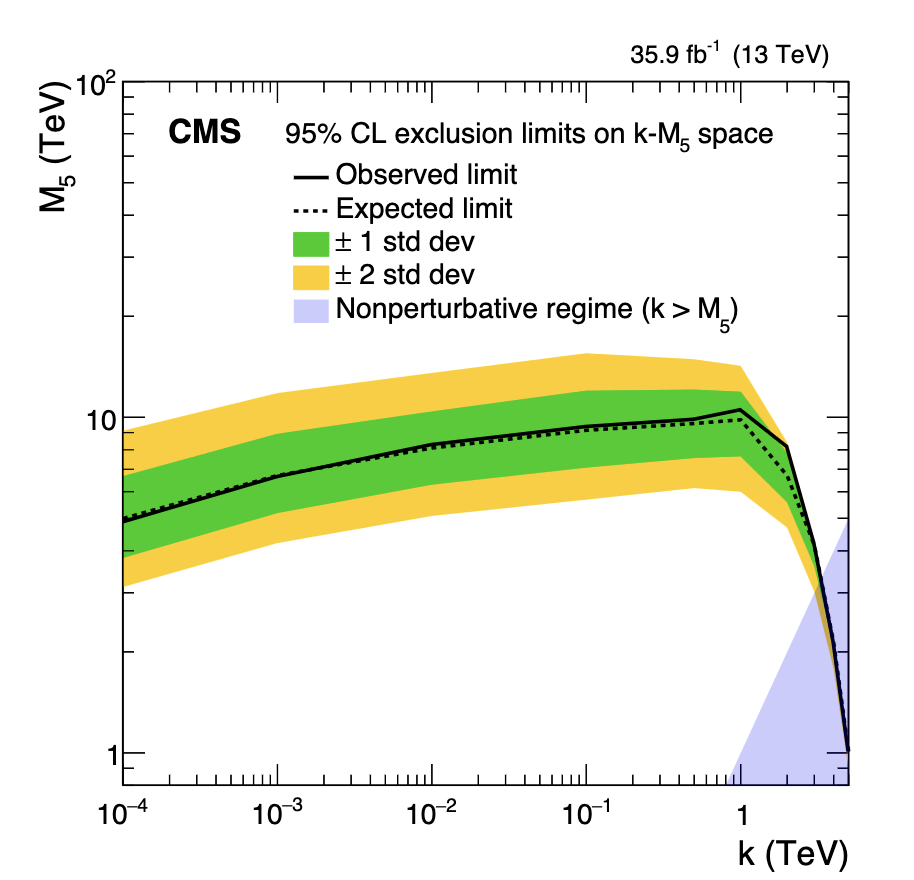
\includegraphics[scale=0.5]{fig/ClockworkCMS.png}
    \caption{The 95\% CL exclusion limits for the continuous graviton model in the clockwork framework over the $k–M_5$ parameter space. The shaded bands represent the 1 and 2 standard deviation uncertainty in the expected limit. The shaded region with $k > M_5$ denotes the area where the theory becomes nonperturbative.}
    \label{fig:ClockworkCMS2016}
\end{figure}


More recently, the ATLAS experiment~\cite{ATLAS:2023hbp} recently placed exclusion limits at 95\% on the two-dimensional parameter space of the clockwork gravity model in their search for periodic signals in the dielectron and diphoton mass spectrum. We compare these recent results with our latest findings in Ch.~\ref{ch:results}.

% \begin{figure}
%     \centering
%     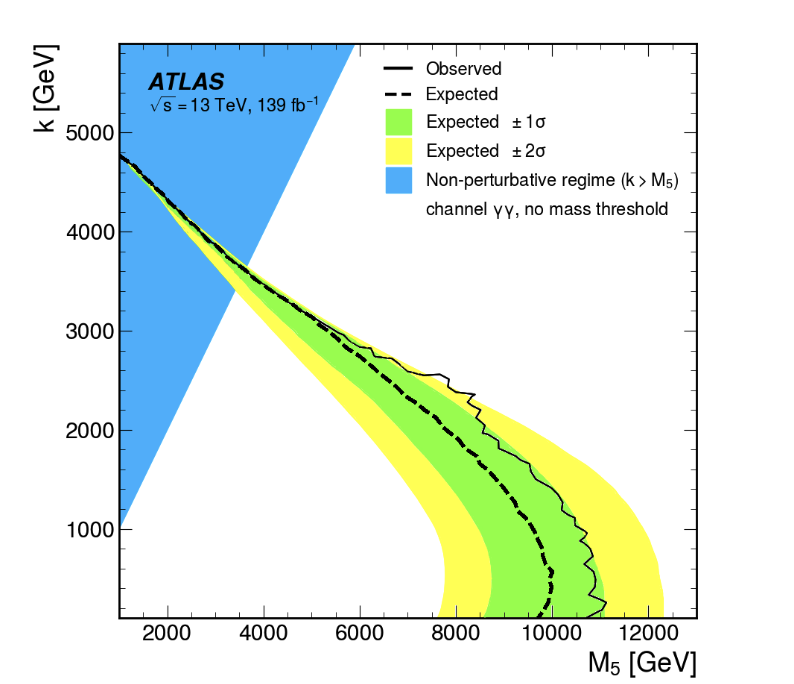
\includegraphics[scale=0.]{fig/ATLASkM5nomass.png}
%     \caption{The expected and observed exclusion limits at 95\% CL for the clockwork gravity model projected in the $k–M_5$ parameter space for the $\gamma\gamma$ channel for the case without mass thresholds. The shaded area with illustrates
% the region of phase space where the CW/LD theory becomes non-perturbative}
%     \label{fig:ATLASLimitsCW}
% \end{figure}

Both the Unparticles and Large Extra dimensions have also been used as additional model interpretations of Searches for Dark Matter that are produced in association with Z boson plus missing $E_{T}$ decays using the full Run II CMS data~\cite{CMS:2020ulv}. While this analysis involves a direct production rather than a virtual exchange of Unparticles, which is what is investigated here. The diphoton channel provides a complementary search where there is potentially more sensitivity for some values of $d_{\mathcal{U}}$ and $\Lambda_{\mathcal{U}}$.

\begin{figure}
    \centering
    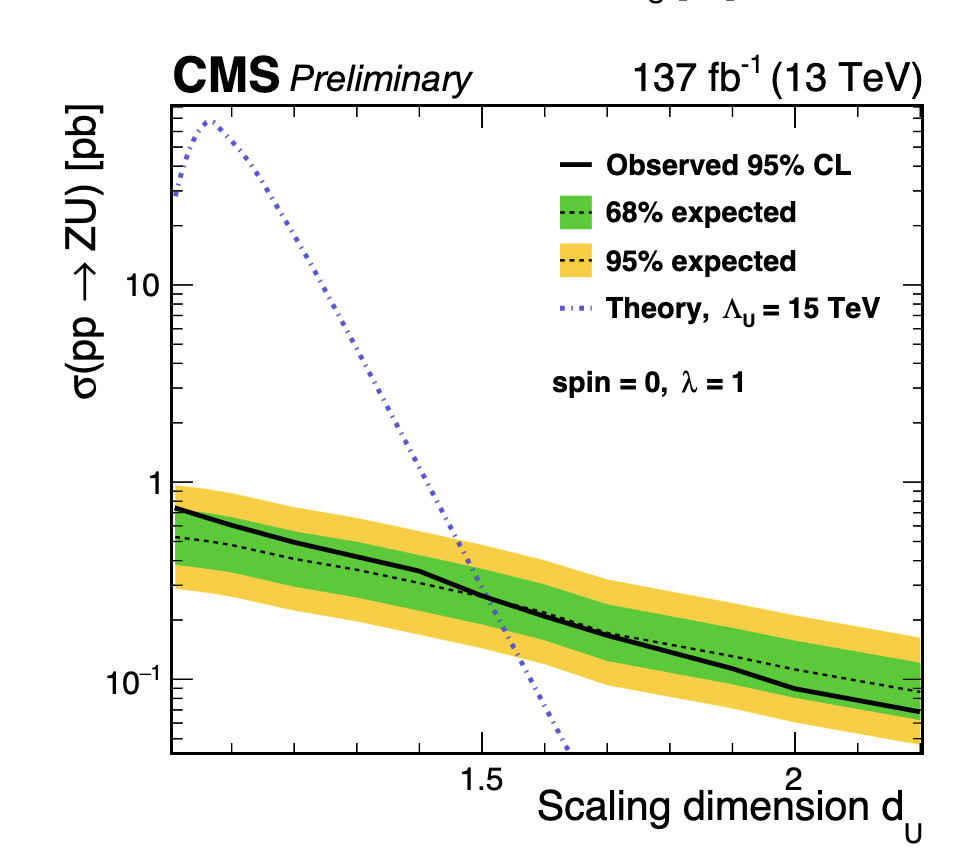
\includegraphics[scale=0.7]{fig/Unparticles.png}
    \caption{The 95\% CL upper limits on unparticle+Z~\cite{CMS:2020ulv} production cross section, as a function of the scaling dimension $d_U$. These limits apply to fixed values of the effective cutoff scale $\Lambda_U$ = 15 TeV and coupling $\lambda$ = 1 }
    \label{fig:UnparZMET}
\end{figure}

\newpage


% \renewcommand{\bibsection}{\topskip=32pt\chapter*{References}\topskip=0pt \addcontentsline{toc}{chapter}{References}\vspace*{6pt}}

% \begin{singlespacing}
% \bibliographystyle{lucas_unsrt.bst}
% \bibliography{references}
% \end{singlespacing}


